%%%%%%%%%%%%%%%%%%%%%%%%%%%%%%%%%%%%%%%%%
% Masters/Doctoral Thesis 
% LaTeX Template
% Version 1.41 (9/9/13)
%
% This template has been downloaded from:
% http://www.latextemplates.com
%
% Original authors:
% Steven Gunn 
% http://users.ecs.soton.ac.uk/srg/softwaretools/document/templates/
% and
% Sunil Patel
% http://www.sunilpatel.co.uk/thesis-template/
%
% License:
% CC BY-NC-SA 3.0 (http://creativecommons.org/licenses/by-nc-sa/3.0/)
%
% Note:
% Make sure to edit document variables in the Thesis.cls file
%
%%%%%%%%%%%%%%%%%%%%%%%%%%%%%%%%%%%%%%%%%

%----------------------------------------------------------------------------------------
%	PACKAGES AND OTHER DOCUMENT CONFIGURATIONS
%----------------------------------------------------------------------------------------

\documentclass[11pt, a4paper, oneside]{Thesis} % Paper size, default font size and one-sided paper

\graphicspath{{Pictures/}} % Specifies the directory where pictures are stored

\usepackage[square, numbers, comma, sort&compress]{natbib} % Use the natbib reference package - read up on this to edit the reference style; if you want text (e.g. Smith et al., 2012) for the in-text references (instead of numbers), remove 'numbers' 
\hypersetup{urlcolor=black, colorlinks=true} % Colors hyperlinks in blue - change to black if annoying
\title{\ttitle} % Defines the thesis title - don't touch this

\begin{document}

\frontmatter % Use roman page numbering style (i, ii, iii, iv...) for the pre-content pages

\setstretch{1.3} % Line spacing of 1.3

% Define the page headers using the FancyHdr package and set up for one-sided printing
\fancyhead{} % Clears all page headers and footers
\rhead{\thepage} % Sets the right side header to show the page number
\lhead{} % Clears the left side page header

\pagestyle{fancy} % Finally, use the "fancy" page style to implement the FancyHdr headers

\newcommand{\HRule}{\rule{\linewidth}{0.5mm}} % New command to make the lines in the title page

% PDF meta-data
\hypersetup{pdftitle={\ttitle}}
\hypersetup{pdfsubject=\subjectname}
\hypersetup{pdfauthor=\authornames}
\hypersetup{pdfkeywords=\keywordnames}

%----------------------------------------------------------------------------------------
%	TITLE PAGE
%----------------------------------------------------------------------------------------

\begin{titlepage}
\begin{center}


\includegraphics[scale=0.1]{Logo} % University/department logo - uncomment to place it 

\textsc{\LARGE \univname}\\[1cm] % University name
\textsc{\Large Final Year Project}\\[0.5cm] % Thesis type

\HRule \\[0.4cm] % Horizontal line
{\huge \bfseries \ttitle}\\[0.4cm] % Thesis title
\HRule \\[1.5cm] % Horizontal line
 
\begin{minipage}{0.4\textwidth}
\begin{flushleft} \large
\emph{Author:}\\
\href{mailto:marcin.baginski91@gmail.com}{\authornames} % Author name - remove the \href bracket to remove the link
\end{flushleft}
\end{minipage}
\begin{minipage}{0.4\textwidth}
\begin{flushright} \large
\emph{Supervisor:} \\
\href{mailto:mike.brookes@imperial.ac.uk}{\supname} % Supervisor name - remove the \href bracket to remove the link  
\end{flushright}
\end{minipage}\\[2cm]
 
\large \textit{This report is submitted in fulfilment of the requirements\\ for the degree of \degreename}\\ % University requirement text
\textit{in the}\\
\deptname\\\univname\\[1.5cm] % Research group name and department name

{\large \today}\\[0.1cm] % Date

 
\vfill
\end{center}

\end{titlepage}

%----------------------------------------------------------------------------------------
%	DECLARATION PAGE
%	Your institution may give you a different text to place here
%----------------------------------------------------------------------------------------

\Declaration{

\addtocontents{toc}{} % Add a gap in the Contents, for aesthetics

I, \authornames, declare that this thesis titled, '\ttitle' and the work presented in it are my own. I confirm that:

\begin{itemize} 
\item[\tiny{$\blacksquare$}] Where any part of this thesis has previously been submitted for a degree or any other qualification at this University or any other institution, this has been clearly stated
\item[\tiny{$\blacksquare$}] Where I have consulted the published work of others, this is always clearly attributed
\item[\tiny{$\blacksquare$}] Where I have quoted from the work of others, the source is always given. With the exception of such quotations, this thesis is entirely my own work
\item[\tiny{$\blacksquare$}] I have acknowledged all main sources of help
\item[\tiny{$\blacksquare$}] Where the thesis is based on work done by myself jointly with others, I have made clear exactly what was done by others and what I have contributed myself \medskip
\end{itemize}
 
Signed:\\
\rule[1em]{25em}{0.5pt} % This prints a line for the signature
 
Date:\\
\rule[1em]{25em}{0.5pt} % This prints a line to write the date
}

\clearpage % Start a new page

%----------------------------------------------------------------------------------------
%	ABSTRACT PAGE
%----------------------------------------------------------------------------------------

\addtotoc{Abstract} % Add the "Abstract" page entry to the Contents

\abstract{\addtocontents{toc}{} % Add a gap in the Contents, for aesthetics

Lorem ipsum dolor sit amet, consectetur adipiscing elit. Maecenas pretium sem nec nisi facilisis, vel consectetur libero rutrum. Curabitur rhoncus commodo leo, nec lobortis ante venenatis vehicula. Duis vel posuere risus. Nulla blandit risus elit, quis eleifend leo lacinia ut. Mauris rutrum vitae orci eu commodo. Suspendisse egestas, ipsum quis interdum rutrum, tortor lectus facilisis lorem, eget mollis ligula arcu at mi. Quisque accumsan orci magna, sit amet interdum lacus commodo non. Mauris elit magna, venenatis in auctor sit amet, laoreet in tortor. Suspendisse et dolor mattis, tempus libero sit amet, tempus lectus. Nunc in dolor et lorem dignissim elementum. Curabitur suscipit lectus lorem. Pellentesque ultrices venenatis neque, vitae consectetur arcu mattis sed. Quisque porta nisl elementum lacus mollis commodo. Sed vestibulum dolor sed lectus interdum eleifend. Quisque in libero ut augue blandit malesuada.
}

\clearpage % Start a new page

%----------------------------------------------------------------------------------------
%	ACKNOWLEDGEMENTS
%----------------------------------------------------------------------------------------

\setstretch{1.3} % Reset the line-spacing to 1.3 for body text (if it has changed)

\acknowledgements{\addtocontents{toc}{\vspace{1em}} % Add a gap in the Contents, for aesthetics

I would like to thank \ldots\medskip
%Last but not least, I would like to thank all my friends and family for their constant support during the time I spent in London. I would have never been able to complete my studies here without you.
}
\clearpage % Start a new page

%----------------------------------------------------------------------------------------
%	LIST OF CONTENTS/FIGURES/TABLES PAGES
%----------------------------------------------------------------------------------------

\pagestyle{fancy} % The page style headers have been "empty" all this time, now use the "fancy" headers as defined before to bring them back

\lhead{\emph{Contents}} % Set the left side page header to "Contents"
\tableofcontents % Write out the Table of Contents

\lhead{\emph{List of Figures}} % Set the left side page header to "List of Figures"
\listoffigures % Write out the List of Figures

%----------------------------------------------------------------------------------------
%	THESIS CONTENT - CHAPTERS
%----------------------------------------------------------------------------------------

\mainmatter % Begin numeric (1,2,3...) page numbering

\pagestyle{fancy} % Return the page headers back to the "fancy" style

% Include the chapters of the thesis as separate files from the Chapters folder
% Uncomment the lines as you write the chapters

%% Chapter Template

\chapter{Introduction} % Main chapter title

\label{Chapter1} % Change X to a consecutive number; for referencing this chapter elsewhere, use \ref{ChapterX}

\lhead{Chapter 1. \emph{Introduction}} % Change X to a consecutive number; this is for the header on each page - perhaps a shortened title

%----------------------------------------------------------------------------------------
%	SECTION 1 - Voice Activity Detection
%----------------------------------------------------------------------------------------

\section{Voice Activity Detection}

Voice Activity Detection (VAD) is a process of identifying parts of an audio recording which contain the presence of human voice as opposed to those which are only comprised of silence or the background noise. VAD is a relatively simple task in recordings which have high signal-to-noise ratios (SNR), in which voice can be distinguished from noise simply by computing the short-time energy of all frames and setting an appropriate threshold for their classification. However, in most modern applications, the signal is almost always corrupted to some extent by a background noise which makes the VAD performance to deteriorate. While some types of noise can be relatively easily dealt with, i.e. those with spectral characteristics different from speech, in the presence of other, it might be very difficult to identify speech segments. One such noise type might be the \emph{babble noise} which consists of speech that we are not interested in. Additionally, VAD decision is especially difficult for the unvoiced phonemes \cite{Kondoz} whose spectrum contains no periodicity and is often similar to the one of white noise \cite{Michaelis}.

There has been an active research in the VAD area from as early as 1975, when Rabiner and Sambur \cite{RabinerSambur} proposed a VAD algorithm (then referred to as \emph{algorithm for determining the endpoints of isolated utterances}) based on the aforementioned short-time energy and the zero-crossing rate. This approach works reasonably well for signals with the SNR on the order of 30 dB and is suitable for a variety of applications which are not subject to a constant, high level of background noise, such as Voice over IP, when a person speaks to a closely positioned microphone in a relatively calm environment. However since then there has been a need for much better performance, including algorithms whose robustness has to be achieved even at negative SNRs. A person driving a car, trying to communicate with their smartphone through its built-in speech recognition system (e.g. Apple Siri) might be one example of such application. Figure \ref{fig:corruptedSpeech} shows a comparison of the amplitude of a clean utterance with the same utterance corrupted by a -5 dB car noise. As it can be seen, some parts of the recording are completely submerged in the noise (especially during the second second of the recording) and their detection poses a considerable challenge for any VAD system. In robotics there is often a desire to communicate with the robot by speaking from a distance which naturally decreases power of the received signal. Taking the detrimental effect of the background noise into consideration, the simple algorithms are likely to either fail completely or their performance might significantly drop.

\begin{figure}[htbp]
	\centering
		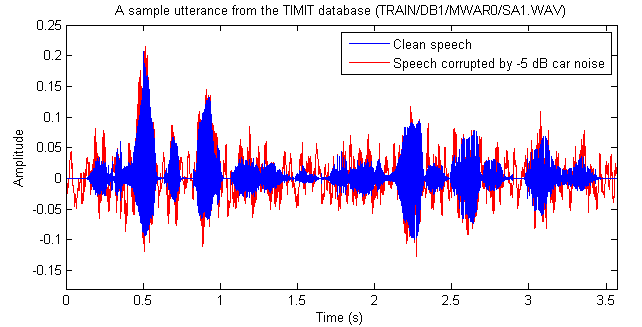
\includegraphics[width=0.9\columnwidth]{Figures/corruptedSpeech.png}
		\rule{37em}{0.5pt}
	\caption[A sample utterance corrupted by -5 dB car noise]{A sample utterance from the TIMIT speech corpus corrupted by -5 dB car noise from the NOISEX-92 database}
	\label{fig:corruptedSpeech}
\end{figure}

%Recently, numerous VAD approaches have been proposed, based on various features such as ..... ..... ..... . 

%----------------------------------------------------------------------------------------
%	SECTION 2 - Applications of VAD 
%----------------------------------------------------------------------------------------

\section{Applications of VAD}

VAD is often the first step in many signal processing applications including speech recognition \cite{RamirezGorriz, Kuroiwa, Martin, Shafran, ImprovedLikelihood, LTSD}, speech coding and transmission \cite{Sohn, RamirezGorriz, Prasad, G729, GSMControl}, speech enhancement \cite{Park, RamirezGorriz, Borisagar}, noise estimation \cite{RamirezGorriz} or speaker recognition \cite{Sahidullah}. In most applications the noise-robust VAD decisions reduce the computational load required by the system and improve its accuracy. The reduced computational load is achieved since the voice-inactive frames are often either transmitted at a much lower bit-rate or not processed at all. At the same time, the clear boundaries of an utterance help to improve the accuracy of some systems (e.g. speech recognition).

\subsection{Automatic Speech Recognition}

In Automatic Speech Recognition (ASR), it is of importance to first extract the voice-active parts of a signal which can then be passed to the actual recognition module. This procedure increases both the accuracy of the ASR system as well as its speed, since the recognition task is not performed on the parts of the signal which do not contain speech. A sample block diagram of an ASR system which uses a VAD module is presented in Figure \ref{fig:ASRVAD} \cite{RamirezGorriz}. For ASR, and also most other applications, it is crucial for the VAD module to be able to identify all speech segments in order not to degrade the accuracy of the entire system. Therefore, VAD systems often implement a fail-safe approach which means that if there is an uncertainty in classification of a frame, it is safer to label is as speech than otherwise. Typically, there is a trade-off in VAD performance which can be characterised as maximising the precision while keeping the recall at a steady, high rate.

\begin{figure}[htbp]
	\centering
		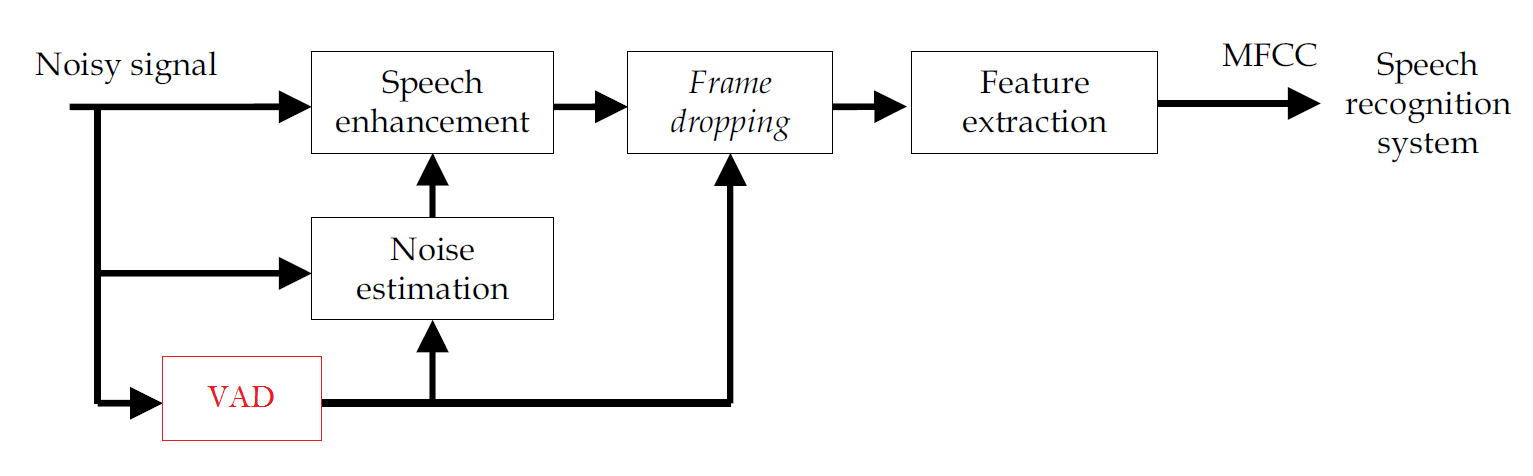
\includegraphics[width=1\columnwidth]{Figures/ASRVAD.png}
		\rule{37em}{0.5pt}
	\caption[Automatic Speech Recognition system with Voice Activity Detection module]{Block diagram of an Automatic Speech Recognition system with Voice Activity Detection module \cite{RamirezGorriz}}
	\label{fig:ASRVAD}
\end{figure}

\subsection{Speech Coding and Transmission}

A typical phone conversation involves each person speaking on average no more than 50\% of the time \citep{GSMControl}. From this fact it can be concluded that signal transmission would be greatly optimised if each transmitter was switched-off half of the time. Such approach could cause the overall system capacity to double. The technique of interrupted transmission during periods of silence is known as discontinuous transmission (DTX). In order to work properly, it requires a precise Voice Activity Detection to direct the operation of a transmitter between being switched on or off. As an alternate method to stopping the transmission, a dual-mode encoding technique could be employed, which uses a higher bit-rate for coding the voice-active frames and lower for silence/noise. The latter is precisely what the popular ITU-T G.729 Annex B \cite{G729} standard does, transmitting the voice-active parts at a fixed bit rate of 8 kb/s while the noisy ones at only 15 b/frame.

Figure \ref{fig:DTXVAD} shows a high-level structure of a dual-mode coding and transmission system, in which the VAD module is used to direct the incoming signal into either the active or inactive speech encoder. The noise can be either transmitted at a much lower bit-rate or the transmission might be switched off completely. In case of a stopped transmission, the receiving end often implements a \emph{comfort noise} \citep{GSMControl,G729,RamirezGorriz} generation module, which creates a synthetic signal similar to the background noise at the transmitter so that the listener does not notice the rapid, inconvenient switching during the conversation.

\begin{figure}[htbp]
	\centering
		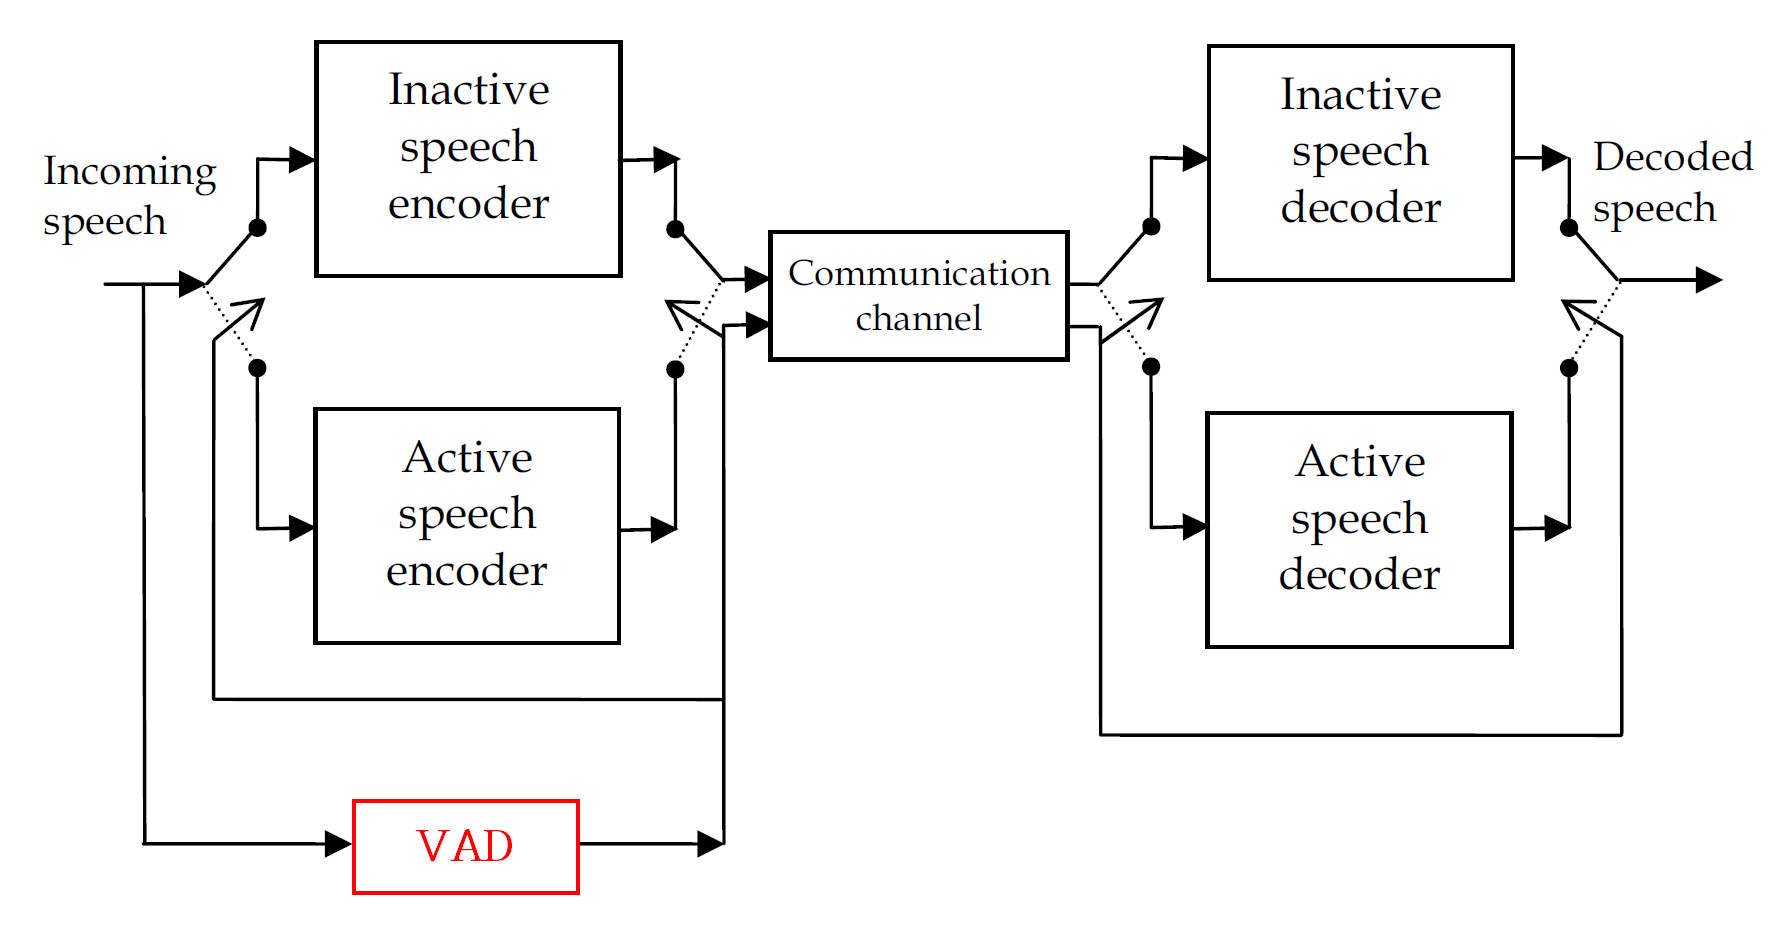
\includegraphics[width=1\columnwidth]{Figures/DTXVAD.png}
		\rule{37em}{0.5pt}
	\caption[Dual-mode transmission system with Voice Activity Detection module]{Block diagram of an dual-mode transmission system with Voice Activity Detection module \cite{G729}}
	\label{fig:DTXVAD}
\end{figure}

\subsection{Noise Estimation and Speech Enhancement}

Speech enhancement aims to improve the intelligibility and quality of speech signals corrupted by additive  noise of some kind. Many speech enhancement systems use a technique called \emph{spectral subtraction} \cite{Kondoz, RamirezGorriz}. It assumes, that the clean speech can be represented in the frequency-domain in the form:
\begin{equation}
|S(f)| = |Y(f)| - |N(f)|
\end{equation}
where $|Y(f)|$ is the amplitude spectrum of the corrupted speech, $|S(f)|$ of the clean speech and $|N(f)|$ of the noise. In order for this technique to work, the noise needs to be additive, stationary and uncorrelated with the clean speech signal. Additionally, one needs to estimate the spectrum of the noise, which in real-world applications where a variety of different, often nonstationary, noise types are encountered, is a nontrivial problem. A robust Voice Activity Detector can become very useful in this task by identifying the voice-inactive frames of a signal from which the noise statistics could be estimated. A precise VAD can also become useful in applications dealing with slowly varying piecewise stationary noises, where the noise statistics can be adaptively estimated based on the most recent VAD decisions.

%----------------------------------------------------------------------------------------
%	SECTION 3 - Structure of a typical VAD system
%----------------------------------------------------------------------------------------

\section{Structure of a typical VAD system}

Figure \ref{fig:VADStructure} shows a high-level structure of a Voice Activity Detector, however only the two middle blocks are considered a core of a typical VAD system.

\begin{figure}[htbp]
	\centering
		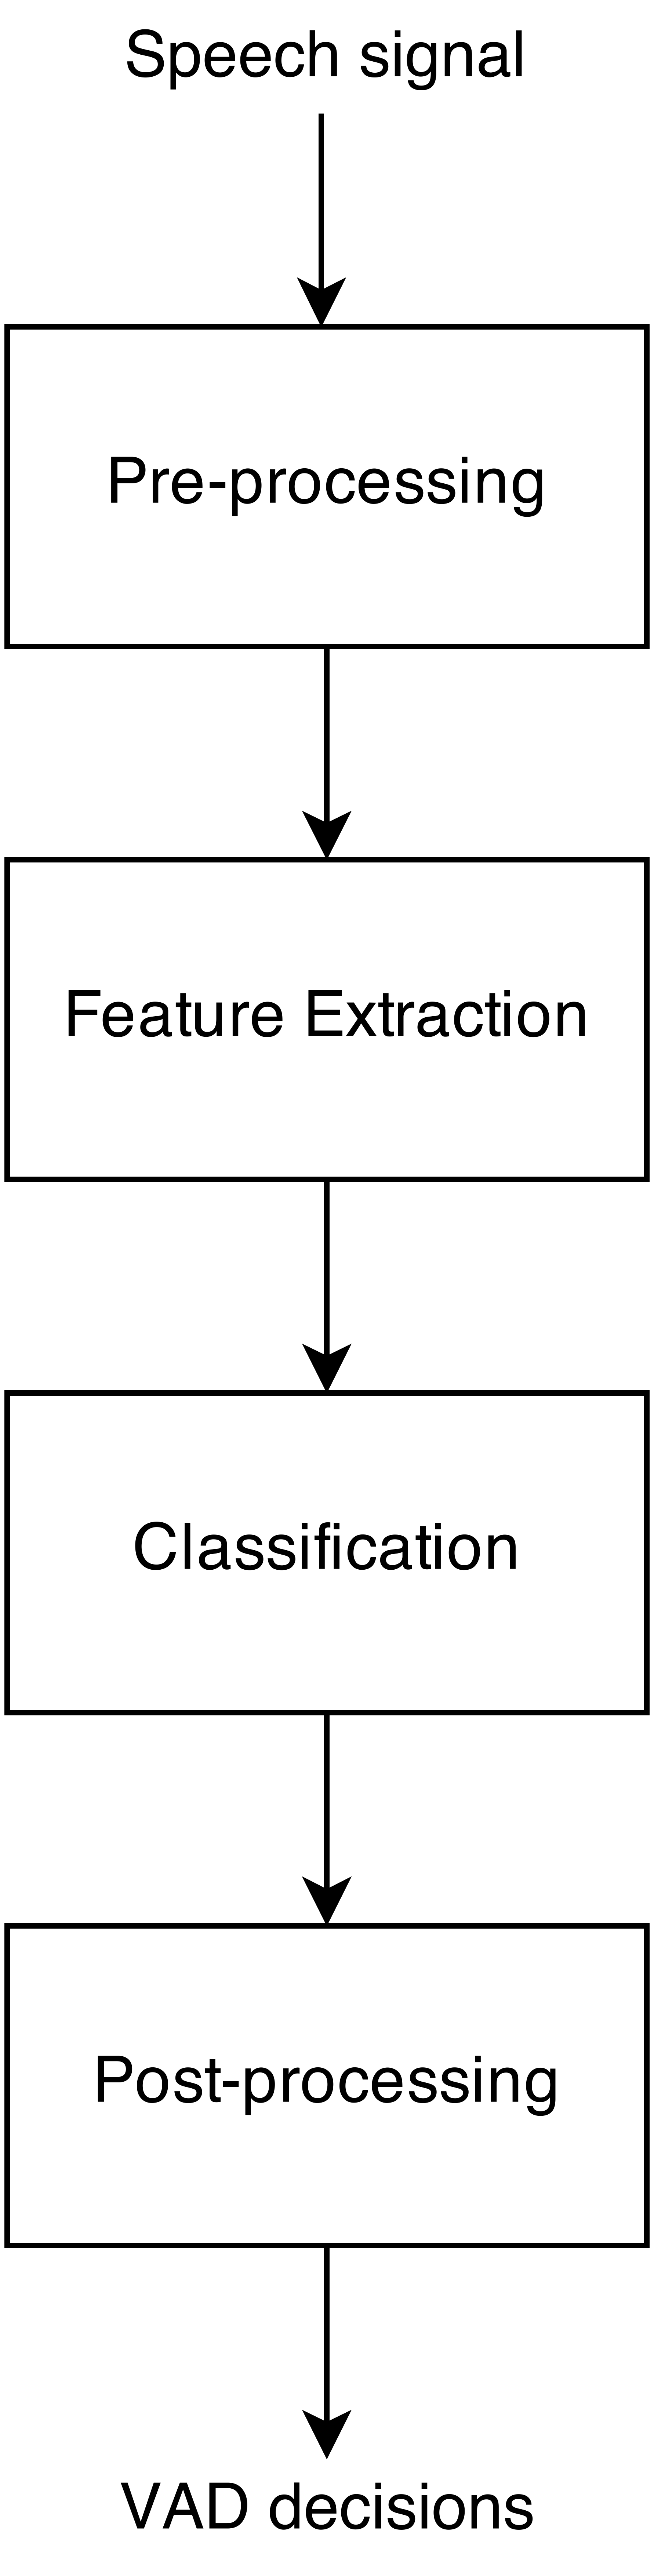
\includegraphics[width=0.15\columnwidth]{Figures/VADStructure2.png}
		\rule{37em}{0.5pt}
	\caption[Block diagram of a typical Voice Activity Detection system]{Block diagram of a typical Voice Activity Detection system}
	\label{fig:VADStructure}
\end{figure}

\subsection{Pre-processing}

The noisy speech signal is first passed to a pre-processing module which might perform a variety of tasks before the actual voice detection takes place. The module might perform noise estimation and suppression in the signal in order to improve performance of the VAD. Additionally, during pre-processing the input signal is often split into frames which are typically 10-50 ms long.

\subsection{Feature Extraction}

The purpose of the feature extraction module is to compute the speech features for each frame which are suitable for the speech/non-speech classification. These can be time-domain \cite{Kida, Weaver}, frequency-domain \cite{Tuske, LTSD}, cepstral-domain \cite{Kotcher} features or other, depending on the specific VAD algorithm. Ideally, in order to achieve the overall VAD system robustness, the selected signal characteristics should not be easily corruptible by the background noise. Additionally, the algorithms for feature extraction should be of low computational complexity for their potential usefulness in real-time applications. The output of this module is therefore a vector $\mathbf{x}$ of features for each of the frames computed in the pre-processing stage.

\subsection{Classification}

The classification module assigns a binary class (speech/non-speech) to each frame based on the feature vector $\mathbf{x}$ received from the previous processing stage. Classification might be based on a variety of decision rules, ranging from simple thresholding \cite{G729} to more advanced methods such as statistical likelihood ratio tests \cite{Sohn, ImprovedLikelihood, SohnInitial} or machine learning \cite{XiaoLei, Stadtschnitzer}. Obviously, the classifier performance degrades with the increasing power of the background noise, therefore there is a need also at this stage for a robust decision making rule. Some researchers \cite{Kida} considered a combination of multiple decision rules in making the final classification.

\subsection{Post-processing}

The last module, post-processing, often tries to \emph{smooth} the VAD decisions (i.e. perform hanging-over) in order to reduce the number of false positives and false negatives. Smoothing is important in order to precisely detect the beginnings and endings of speech bursts, which often have much lower energy than the rest of the signal. Additionally, if among 50 consecutive frames, each of 20 ms duration, only one is classified as speech, the post-processing module might change the decision for this particular frame, since it is highly unlikely for speech to be active during such short-time window. The hang-over schemes  proposed in the literature are often based on simple heuristics \cite{G729} or other techniques such as Hidden Markov models \cite{Sohn}.

%----------------------------------------------------------------------------------------
%	SECTION 4 - Thesis organisation
%----------------------------------------------------------------------------------------

\section{Thesis organisation}

The rest of this document is organised as follows:
\begin{itemize}
\item Chapter 2 contains a literature survey of both the standardised as well as recently proposed VAD algorithms from various sources such as conference proceedings or scientific journals
\item Chapter 3 presents an evaluation of selected VAD algorithms from Chapter 2 on the TIMIT speech corpus corrupted by various noise types from the NOISEX-92 database
\item 
\end{itemize}
%% Chapter Template

\chapter{Literature Survey of VAD algorithms} % Main chapter title

\label{Chapter2} % Change X to a consecutive number; for referencing this chapter elsewhere, use \ref{ChapterX}

\lhead{Chapter 2. \emph{Literature Survey of VAD algorithms}} % Change X to a consecutive number; this is for the header on each page - perhaps a shortened title

%----------------------------------------------------------------------------------------
%	SECTION 1 - Standard VAD algorithms
%----------------------------------------------------------------------------------------

\section{Standard VAD algorithms}
\label{sec:StandardVADs}

Being an important tool in many speech processing applications, a number of VAD algorithms have been subject to standardisation by various organisations such as the International Telecommunication Union (ITU-T), European Telecommunications Standards Institute (ETSI), Telecommunications Industry Association (TIA) or Electronic Industries Alliance (EIA). Most standardised algorithms use the energy of the input signal as a Voice Activity Detection feature. It is important to note that the standardised VAD approaches have been developed for use in the telecommunications industry, with particular emphasis on the application for discontinuous transmission (DTX), which may make them less appropriate for other speech processing tasks such as speech recognition. Nevertheless, these algorithms often serve as a benchmark for the newly developed VAD features, whose performance is often compared to the standard ones.

In the rest of this section, three standard VAD algorithms are going to be described:
\begin{itemize}
\item ITU-T G.729 Annex B \citep{G729} which is an extension to the G.729 speech coder with an aim to achieve an improved bit rate during the noise-only periods
\item ETSI AMR1 and AMR2 \cite{AMR} for application to the Global System for Mobile Communications (GSM)
\item TIA/EIA IS-733 \cite{IS733} for application to the Wideband Spread Spectrum Communication Systems
\end{itemize}

\subsection{ITU-T G.729 Annex B}

The well-known ITU-T G.729 Annex B VAD has been developed as an extension to the G.729 speech coding algorithm \citep{G729Original} transmitting each frame at a fixed bit rate of 8 kb/s. Application of the Voice Activity Detector allows to identify the noise-only frames in a continuous stream of data and adopt a compressed transmission at only 15 b/frame which contains information about the background noise for reproduction by the Comfort Noise Generator (CNG) at the receiving end. This approach for speech/noise coding allows to reduce the average bit-rate of the entire coder from 8 kb/s to only 4 kb/s while keeping the transmission quality unchanged.

The block diagram of the VAD algorithm is presented in Figure \ref{fig:G729AnnexB}. It starts with computation of four main \emph{instantaneous parameters} for the current frame which describe the energy and spectral content of the signal:
\begin{itemize}
\item Set of Line Spectral Frequencies (LSF)
\item Full-band energy ($E_f$)
\item Low-band (0 to 1 kHz) energy ($E_l$)
\item Zero-crossing rate (ZCR)
\end{itemize}

\begin{figure}[htbp]
	\centering
		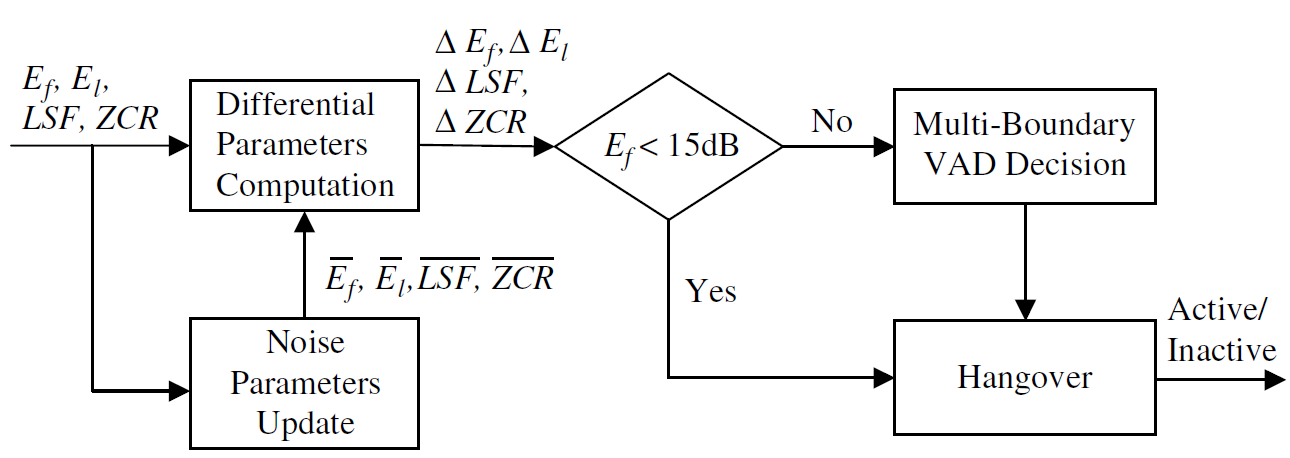
\includegraphics[width=0.9\columnwidth]{Figures/Chapter2/G729AnnexB.png}
		\rule{37em}{0.5pt}
	\caption[Block diagram of the ITU-T G.729 Annex B VAD]{Block diagram of the ITU-T G.729 Annex B VAD \cite{Kondoz}}
	\label{fig:G729AnnexB}
\end{figure}

The \emph{instantaneous parameters} are then differenced with their most recent average noise-only counterparts in order to derive an additional set of so called \emph{difference parameters} which are used for speech/non-speech classification. The set of all possible \emph{difference parameters} describes a four dimensional Euclidean space in which a specific region contains the speech frames while another region describes the noise-only frames. The current vector of parameters is compared against the pre-computed regions in order to classify the current frame. The two regions are initially identified by visual inspection of the points' distribution over a large set of clean and noisy recordings. An energy threshold of $E_f < 15$ dB is applied before the multi-boundary classification in order to minimise short glitches on low-energy frames.

ITU-T G.729 Annex B uses an additional four-step heuristic-based smoothing scheme after the initial multi-boundary classification:
\begin{enumerate}
\item An active voice decision is extended to the current frame if its energy is above a certain threshold
\item An active voice decision is extended to the current frame if the previous two frames were speech and the absolute energy difference between the current and previous frames' is under a certain threshold
\item An inactive voice decision is extended to the current frame if the previous 10 frames were noise-only and the absolute energy difference between current and previous frames' is under a certain threshold
\item The active voice frame is labelled as inactive if the current frame energy is below a noise floor by a certain threshold
\end{enumerate}

The main VAD algorithm also performs updating of the noise parameters ($\overline{LSF}$, $\overline{E_f}$, $\overline{E_l}$ , $\overline{ZCR}$) by a secondary VAD decision which does not need to be as robust as the primary one since it is used only for estimation of the noise parameters.

\subsection{ETSI AMR1 and AMR2}

ETSI proposed two VAD alternatives for use in the Adaptive Multi-Rate speech traffic channels. In both algorithms, the decision is primarily based on the energy of the signal across different frequency bands.

A block diagram of the AMR Option 1 VAD is presented in Figure \ref{fig:AMR1}. The original algorithm includes additional processing steps to those depicted in the Figure in order to determine whether the incoming signal, if not noise-only, contains speech, special information tone (STI) or other (e.g. music), however this details are are omitted in this description.

\begin{figure}[htbp]
	\centering
		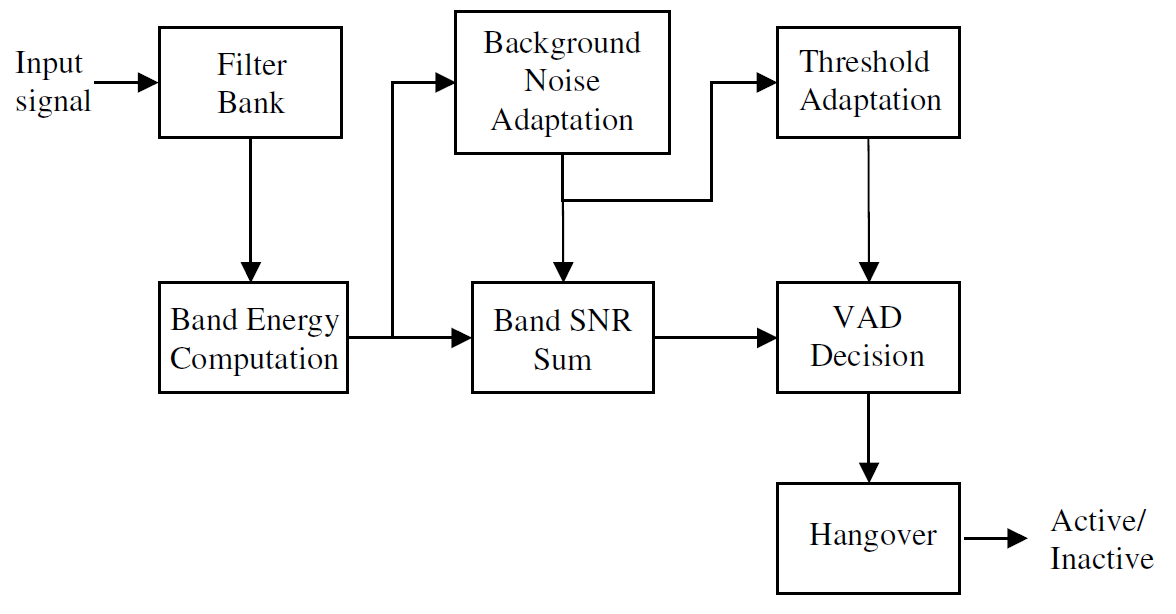
\includegraphics[width=0.9\columnwidth]{Figures/Chapter2/AMR1.png}
		\rule{37em}{0.5pt}
	\caption[Block diagram of the ETSI AMR Option 1 VAD]{Block diagram of the ETSI AMR Option 1 VAD \cite{Kondoz}}
	\label{fig:AMR1}
\end{figure}

The input signal is first passed through a series of nine band-pass filters which split the time-domain signal into different frequency bands based on the Table \ref{tab:AMR1filterbank}. The signal level $level[n]$ is calculated at the output of each filter as a sum of the absolute values of all samples in the current frame. The VAD feature is then computed according to the Equation \ref{eq:AMR1SNR}

\begin{equation}
\text{SNR} = \sum_{n=1}^{9} \max (1.0, \frac{level[n]}{bckr\_est[n]})^{2} 
\label{eq:AMR1SNR}
\end{equation}

where $bckr\_est[n]$ is the estimated level of noise at frequency band $n$. The VAD feature from the above equation is compared to a threshold in order to classify the current frame. The threshold is determined based on the estimated average background noise level which is the sum of $bckr\_est[n]$ for all $n$. As a final processing step, AMR Option 1 VAD includes a hang-over scheme in order to detect the low-energy endings of speech bursts.

\begin{table}[htbp]
\center
\begin{tabular}{c|c|}
\cline{2-2}
 & Frequencies \\ \hline
\multicolumn{1}{ |c| }{Filter 1} & 0 - 250 Hz \\ \hline
\multicolumn{1}{ |c| }{Filter 2} & 250 - 500 Hz \\ \hline
\multicolumn{1}{ |c| }{Filter 3} & 500 - 750 Hz \\ \hline
\multicolumn{1}{ |c| }{Filter 4} & 750 - 1000 Hz \\ \hline
\multicolumn{1}{ |c| }{Filter 5} & 1000 - 1500 Hz \\ \hline
\multicolumn{1}{ |c| }{Filter 6} & 1500 - 2000 Hz \\ \hline
\multicolumn{1}{ |c| }{Filter 7} & 2000 - 2500 Hz \\ \hline
\multicolumn{1}{ |c| }{Filter 8} & 2500 - 3000 Hz \\ \hline
\multicolumn{1}{ |c| }{Filter 9} & 3000 - 4000 Hz \\ \hline
\end{tabular}
\caption[Cut-off frequencies for the ETSI AMR1 band-pass filters]{Cut-off frequencies for the ETSI AMR1 band-pass filters \citep{AMR}}
\label{tab:AMR1filterbank}
\end{table}

A block diagram of ETSI AMR Option 2 VAD is presented in Figure \ref{fig:AMR2}. The concept is similar to Option 1 VAD, however the incoming signal is split into different frequencies not by time-domain band-pass filtering, but by first computing the Discrete Fourier Transform (DFT) of the signal and performing further analysis in the frequency domain. The frequencies are clustered into bands (channels) and the energy of each channel is calculated \citep{Cornu}. In the next processing steps, SNR of each channel is calculated and transformed to a \emph{voice metric} by a specific function which results in the final VAD feature to be classified by using a threshold. An additional part of the system performs updates of the noise statistics based on the spectral deviation estimate.

\begin{figure}[htbp]
	\centering
		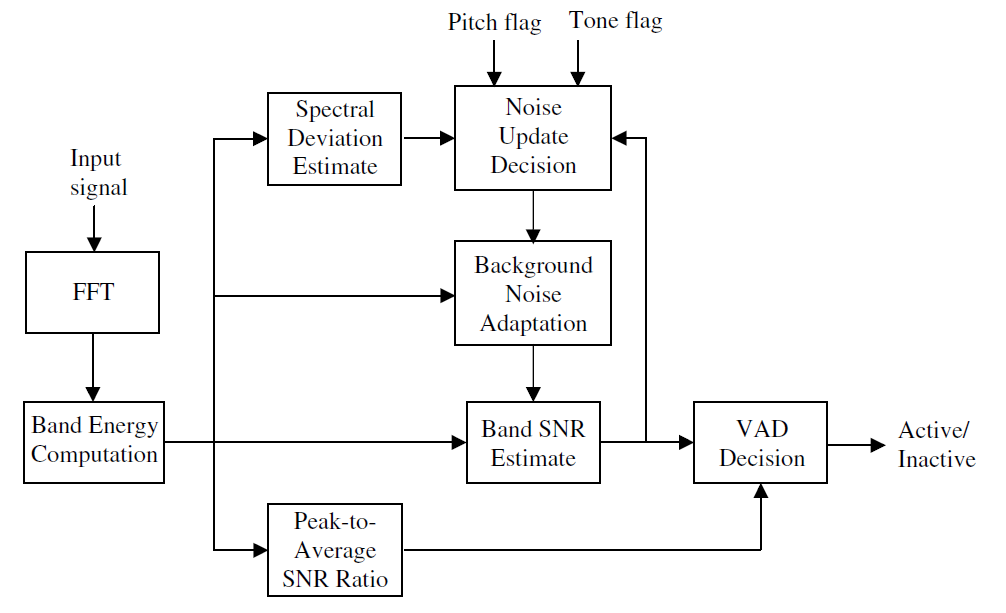
\includegraphics[width=0.9\columnwidth]{Figures/Chapter2/AMR2.png}
		\rule{37em}{0.5pt}
	\caption[Block diagram of the ETSI AMR Option 2 VAD]{Block diagram of the ETSI AMR Option 2 VAD \cite{Kondoz}}
	\label{fig:AMR2}
\end{figure}

\subsection{TIA/EIA IS-733}

TIA/EIA IS-733 is a speech coder in which the signal might be encoded at four different rates ($1$, $\frac{1}{2}$, $\frac{1}{4}$, $\frac{1}{8}$ of the base rate) depending on the characteristics of the currently transmitted frame. Rate $1$ is used for low quality signals where additional reduction might compromise the already low intelligibility. Rate $\frac{1}{2}$ is used for good quality stationary and periodic frames. Rate $\frac{1}{4}$ is used for unvoiced speech and rate $\frac{1}{8}$ for speech inactive frames. A VAD algorithm is used to determine the rate at which the current frame should be encoded and transmitted.

A block diagram of TIA/EIA IS-733 VAD is presented in Figure \ref{fig:IS733}. The algorithm starts with computing the energy of the input signal across two different frequency bands (0.3 - 2.0 kHz and 2.0 - 4.0 kHz) and subsequently the SNR based on the estimated noise energy. The VAD decision is based on two adaptive thresholds, which depend on the level of the estimated background noise, one for each frequency band. If both low and high band SNRs are higher than the threshold, rate 1 is selected. Only one SNR being above its threshold causes the signal to be encoded at rate $\frac{1}{2}$. Both SNRs below the threshold indicate noise-only frame, encoded at rate $\frac{1}{8}$.

\begin{figure}[htbp]
	\centering
		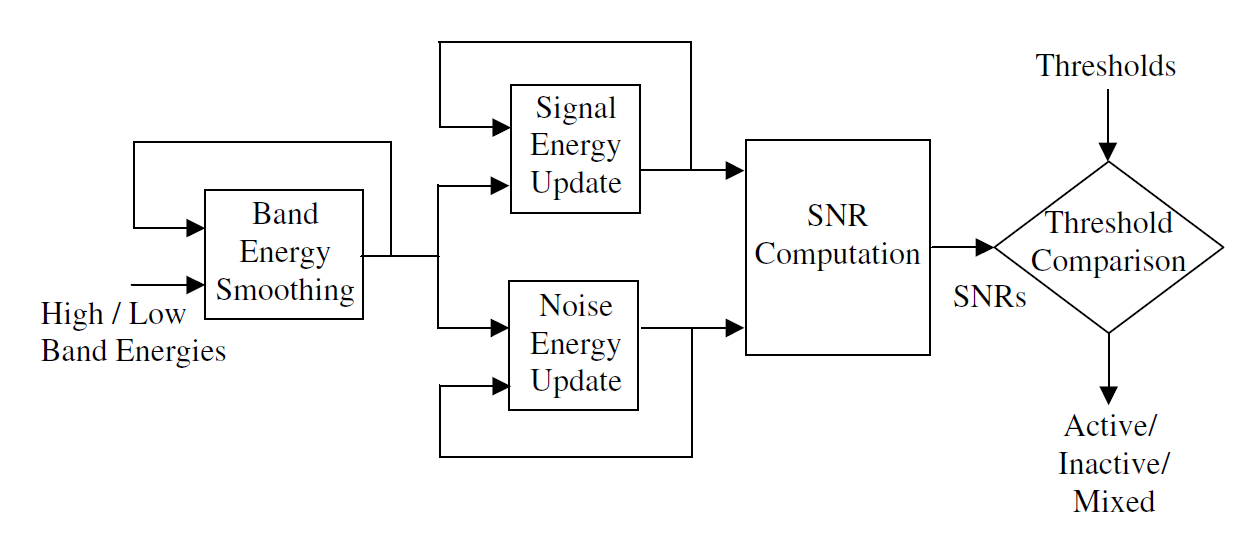
\includegraphics[width=0.9\columnwidth]{Figures/Chapter2/IS733.png}
		\rule{37em}{0.5pt}
	\caption[Block diagram of the TIA/EIA IS-733 VAD]{Block diagram of the TIA/EIA IS-733 VAD \cite{Kondoz}}
	\label{fig:IS733}
\end{figure}

\subsection{Summary}

Some VAD algorithms have been standardised by various telecommunication standards institutes (ITU-T, ETSI, TIA/EIA). Those algorithms are predominantly based on simple features such as the energy of the signal or the zero-crossing rate, sometimes across different frequency ranges. While such measures are often sufficient to meet the requirements of the high SNR transmission found in telecommunications, their performance drops significantly with the increased power of noise. Nevertheless, the standard algorithms serve as a convenient benchmark for the more recently proposed VAD features, described in section \ref{sec:RobustVADs} which are aimed to be more noise-robust and useful in other speech processing tasks.

%----------------------------------------------------------------------------------------
%	SECTION 2 - Noise-robust VAD algorithms
%----------------------------------------------------------------------------------------

\section{Noise-robust VAD algorithms}
\label{sec:RobustVADs}

Apart from standard VAD algorithms described in section \ref{sec:StandardVADs}, many independent researchers have made numerous attempts to develop novel noise-robust Voice Activity Detection methods. Most of these research results either in invention of the new features or identification of ways in which the existing ones might be improved. Ideally, the most robust feature should have no common values for the noise and speech frames. Figure \ref{fig:featureDist} shows the distribution of values for some of the features used by algorithms described in this section for the clean speech from the TIMIT \cite{TIMIT} database and a variety of noise types from the NOISEX-92 \cite{NOISEX} database. It is clear, that in both cases the values for the clean speech are mostly distinct from the ones for noise frames, however there is still much overlap between them which indicates a room for improvement.

\begin{figure}[htbp]
	\centering
		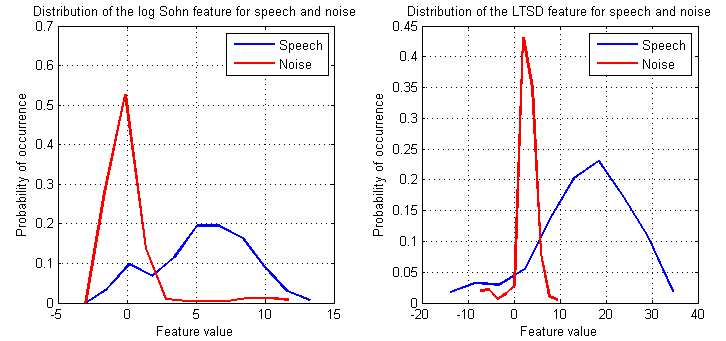
\includegraphics[width=0.9\columnwidth]{Figures/Chapter2/featureDist.png}
		\rule{37em}{0.5pt}
	\caption[Distribution of Sohn's and LTSD features for speech and noise]{Distribution of Sohn's \cite{SohnInitial} and LTSD \cite{LTSD} features for speech and noise}
	\label{fig:featureDist}
\end{figure}

\subsection{Entropy-based VAD}

In contrast to the standardised energy-based methods, some researchers investigated the idea of using entropy for Voice Activity Detection. Entropy, as originally defined by Shannon \cite{Shannon}, is a measure of uncertainty in a random variable, given by the equation:

\begin{equation}
E = - \sum_{i=1}^{N} p_i \log_2 p_i
\label{eq:entropy}
\end{equation}

where $p_i$ is the probability of the random variable having a value of $i$ among $N$ distinct values which it might take. In case of VAD, $p_i$ often relates to either a single bin in a histogram of the amplitudes of a signal or a single frequency in the magnitude power spectrum.

The purely time domain approach to VAD using entropy has been explored by Weaver \emph{et al.} in \cite{Weaver}. A block diagram of the key parts of the algorithm is presented in Figure \ref{fig:Weaver}. The authors propose to first calculate the histogram of the amplitudes of the signal and then assign an entropy measure to each frame, as defined in Equation \ref{eq:entropy}, where $p_i$ is the normalised (such that $\sum_{i=1}^{N} p_i = 1$) mass of the $i$-th bin of the histogram.

\begin{figure}[htbp]
	\centering
		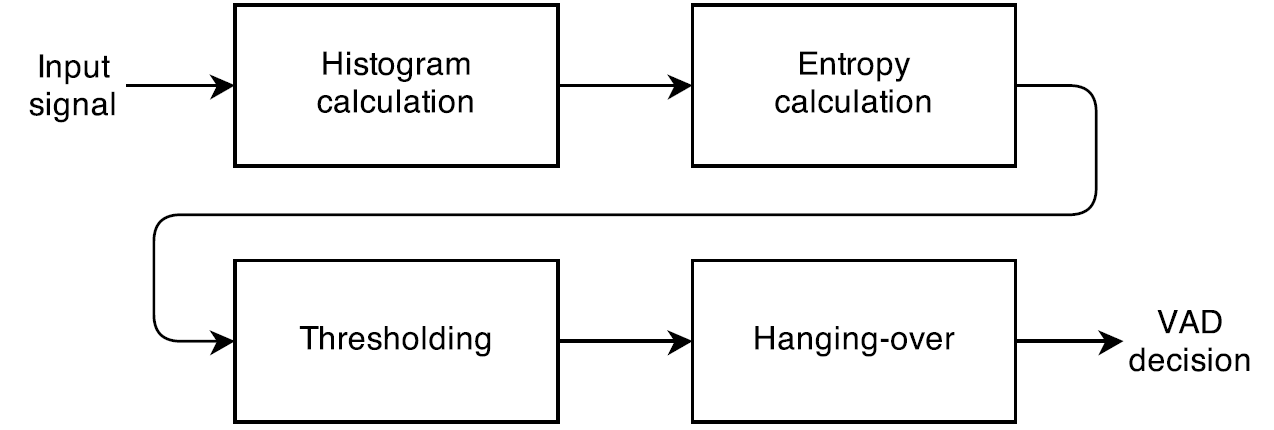
\includegraphics[width=0.9\columnwidth]{Figures/Chapter2/Weaver.png}
		\rule{37em}{0.5pt}
	\caption[Block diagram of the time-domain entropy-based VAD]{Block diagram of the time-domain entropy-based VAD \cite{Weaver}}
	\label{fig:Weaver}
\end{figure}

While this approach is more noise-robust than the simple energy-based methods, especially for the stationary narrowband noise types, its performance is significantly affected by the various coloured noises. In order to mitigate this weakness, the authors propose to use a weighting filter in order to enhance the typical speech frequencies, however it needs to be kept in mind that if we are faced with a noise with spectral characteristics very similar to speech (especially in case of the \emph{babble noise}), the filter would become essentially useless as it would emphasise the noise as well.

A frequency domain approach to using entropy for VAD has been considered by Renevey \emph{et al.} in \cite{Renevey}. Instead of first computing the histogram of the amplitudes of the input signal, the frequency-domain algorithm starts with calculating the power spectrum of each frame. Entropy of the spectrum is then calculated by means of the following equation:

\begin{equation}
E( \left |  Y \left ( \omega, t \right ) \right |^{2} ) = - \sum_{i=1}^{L} P( \left |  Y \left ( \omega_i, t \right ) \right |^{2} ) \log \left( P( \left |  Y \left ( \omega_i, t \right ) \right |^{2} ) \right)
\end{equation}

where $P( \left |  Y \left ( \omega_i, t \right ) \right |^{2} )$ denotes the fraction of the sum of all harmonics which is attributable to the current frequency $i$.

\begin{figure}[htbp]
	\centering
		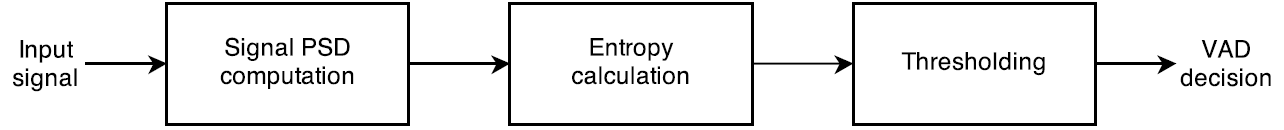
\includegraphics[width=0.9\columnwidth]{Figures/Chapter2/Renevey.png}
		\rule{37em}{0.5pt}
	\caption[Block diagram of the frequency-domain entropy-based VAD]{Block diagram of the frequency-domain entropy-based VAD \cite{Renevey}}
	\label{fig:Renevey}
\end{figure}

All entropy-based approaches to VAD are most effective for the white noise and alike, since the distribution of entropy for speech is much different from the one for noise. The completely unpredictable nature of white noise yields high entropy values, while the more organised and predictable clean speech signals present a naturally lower entropy. Both the time and frequency domain algorithms' performance drops significantly for a variety of coloured noise types. In order to improve the performance for in such environments, the authors of \cite{Renevey} propose using a \emph{whitening} filter which divides the spectrum of the current frame by an average of all frames.

\subsection{Likelihood Ratio Test VAD}
\label{ssec:LRT}

`A Statistical Model-Based Voice Activity Detector' proposed by Sohn \emph{et al.} \cite{Sohn} is one of the most widely cited VAD algorithms due to its ease of implementation, robustness and extensibility. The idea of using a Likelihood Ratio Test (LRT) has been considered by many other researchers who tried to improve on the original approach \cite{ImprovedLikelihood, Cho}. The initial algorithm has been developed in \cite{SohnInitial} and extended to improve noise-robustness in \citep{Sohn}. A block diagram of Sohn's VAD is presented in Figure \ref{fig:Sohn}.

\begin{figure}[htbp]
	\centering
		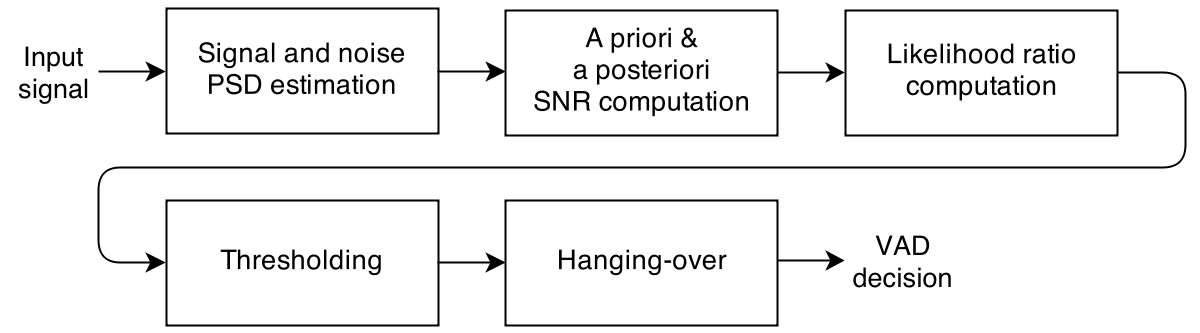
\includegraphics[width=0.9\columnwidth]{Figures/Chapter2/Sohn.png}
		\rule{37em}{0.5pt}
	\caption[Block diagram of the Statistical Model-Based VAD]{Block diagram of the Statistical Model-Based VAD \cite{Sohn}}
	\label{fig:Sohn}
\end{figure}

The algorithm is based on a LRT to discriminate between two hypotheses:
\begin{itemize}
\item[] $H_0$ - speech absent
\item[] $H_1$ - speech present
\end{itemize}

The measure which is used for the preliminary VAD decision (i.e. before the hang-over scheme) is a combination of the likelihood ratios from each frequency bin $k$:

\begin{equation}
\log \Lambda = \frac{1}{L} \sum_{k=0}^{L-1} \log \frac{1}{1+\xi_k} e^{\frac{\gamma_k\xi_k}{1+\xi_k}}
\end{equation}

where $L$ is the number of samples in each frame, $\xi_k$ is the \emph{a priori} SNR and $\gamma_k$ is the \emph{a posteriori} SNR. In order for the algorithm to work, one needs to obtain the values for $\xi_k = \frac{\left | S_k \right |^{2}}{\left | N_k \right |^{2}}$ and $\gamma_k = \frac{\left | X_k \right |^{2}}{\left | N_k \right |^{2}}$ where $\left | X_k \right |^{2}, \left | S_k \right |^{2}, \left | N_k \right |^{2}$ are the PSDs of the noisy speech, clean speech and noise respectively. $\left | N_k \right |^{2}$ can be obtained by means of any noise estimation procedure (e.g. \cite{MSnoise} or \cite{MMSEnoise}), whose accuracy influences the noise robustness of the algorithm. The VAD feature is thresholded by an empirically determined constant for the preliminary decision. Finally, the authors proposed a Hidden Markov model (HMM) hang-over scheme in order to improve accuracy of the algorithm for the low-energy beginnings and endings of the speech utterances.

While the original idea to the derivation of the unknown \emph{a priori} SNR $\xi_k$ involved the Maximum Likelihood estimator $\xi_k^{ML} = \gamma_k - 1$, in \cite{Sohn} a limitation of the procedure has been identified which makes it biased towards $H_1$. In an effort to improve the algorithm, the authors proposed a decision-directed (DD) estimation procedure which reduces the fluctuation of the likelihood ratios by using a MMSE short-time spectral amplitude estimator \cite{Ephraim} and a first-order low pass filter.

In an effort to further improve the LRT-based algorithm, Cho \emph{et al.} \cite{Cho} investigated the DD approach with particular interest in the detection errors occurring at the endings of speech utterances. It was determined that the frequent misdetections are due to the delay in the DD \emph{a priori} SNR estimator, which prevents the estimated value to drop quick enough for the likelihood ratio to stay above the threshold during the short, low-energy speech offset regions. In order to alleviate this problem, the authors proposed a smoothed likelihood ratio (SRT), which delays the sudden drops in the LR at the speech offset regions due to the constant $\alpha \approx 0.9$. The SRT is defined in Equation \ref{eq:SRT} where $n$ relates to the frame number while $k$ is the frequency bin. The final VAD decision is calculated by taking a geometric mean of the SRTs from all frequency bins.

\begin{equation}
\Phi (n,k) = \exp \left\{ \alpha \log \left( \Phi (n-1,k) \right) + (1-\alpha) \log \left( \Lambda (n,k) \right) \right\}
\label{eq:SRT}
\end{equation}

Both \cite{Sohn} and \cite{Cho} VAD methods consider only a single frame when making a speech/non-speech decision and hence they are likely to misclassify the low-energy frames for which the short-time SNR is much lower than the average SNR of the entire signal. To aid the proper detection of such frames, in \cite{RamirezMulti} Ramirez \emph{et al.} proposed a multiple observation vector which considers $M$ frames before and ahead of the current frame in formulating the likelihood ratio. The main rationale behind this idea is that the weaker speech frames are often surrounded by the stronger parts, and their inclusion in the LRT might boost its value above the threshold. While this approach results in somewhat improved performance, it also introduces the delay of $M$ frames to the algorithm, which might prevent it from being used in some real-time applications.

\subsection{Long-Term Spectral Divergence VAD}

Another popular and widely cited algorithm is the Ramirez \emph{et al.} \cite{LTSD} VAD based on the long-term speech information. The main assumption of the algorithm is that the most discriminative speech/non-speech information lies on the shape of the magnitude spectrum of the analysed signal. However, instead of considering each frame independently, the algorithm also includes the information contained in the neighbouring frames. The reason behind that is to boost the detection of the low-energy unvoiced phonemes which are typically surrounded by the high-energy voiced ones. Therefore, it can be said that the LTSD algorithm uses an implicit hang-over scheme incorporated directly in the voicing feature.

The algorithm starts by computing the so-called long-term spectral envelope (LTSE) which uses information contained in the current frame as well as $N$ preceding and succeeding frames i.e. $2N+1$ frames in total for every calculation. Based on the LTSE, the long-term spectral divergence (LTSD) is calculated which serves as the VAD decision rule. In Ramirez's study, it has been established that the best performance is achieved for $N=6$ however this value is likely to be dependent on the particular application as well as the level of noise.

\begin{figure}[htbp]
	\centering
		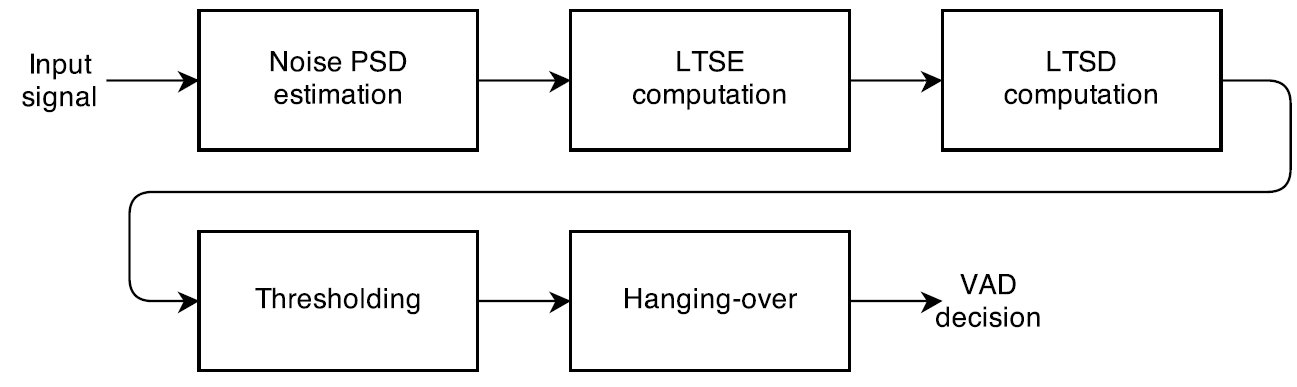
\includegraphics[width=0.9\columnwidth]{Figures/Chapter2/LTSD.png}
		\rule{37em}{0.5pt}
	\caption[Block diagram of the Long-Term Spectral Divergence VAD]{Block diagram of the Long-Term Spectral Divergence VAD \cite{LTSD}}
	\label{fig:LTSD}
\end{figure}

A block diagram of the LTSD-based VAD is presented in Figure \ref{fig:LTSD}. The algorithm starts with an assumption that the first $N$ frames of each utterance do not contain any speech and that the average magnitude spectrum of the noise can be estimated from them. After that, the LTSE for each frame is computed according to Equation \ref{eq:LTSE} where $X(k,l)$ is the amplitude spectrum at frequency $k$ for frame $l$.

\begin{equation}
\text{LTSE}(k,l) = \max \left \{ X(k,l-N),\ldots,X(k,l),\ldots,X(k,l+N) \right \}
\label{eq:LTSE}
\end{equation}

The LTSD is obtained from Equation \ref{eq:LTSD} where $M$ is the number of frequency bins in the DFT and $N(k)$ is the average noise amplitude spectrum at frequency $k$ as estimated before. Essentially what the equation describes is the average deviation of the LTSE from the noise statistics at each frequency bin. In other words, this measure might be interpreted as a variation of the estimated \emph{a posteriori} signal-to-noise ratio, which is an idea exploited in many VAD algorithms.

\begin{equation}
\text{LTSD}(l) = 10 \log_{10} \left ( \frac{1}{M} \sum_{k=0}^{M-1} \frac{\text{LTSE}^{2}(k,l)}{N^{2}(k)} \right )
\label{eq:LTSD}
\end{equation}

Eventually, the LTSD feature is thresholded to form a preliminary VAD decision which might be further revised by a separate hang-over scheme.

\subsection{Pitch and fundamental frequency based VAD}

A rather unique feature of the voiced speech is its spectral harmonicity. The magnitude spectrum of the voiced phonemes contains clearly visible peaks at equal intervals corresponding to the fundamental frequency $F_0$ or pitch; the terms which in speech processing context are often used interchangeably. A spectrogram of a sample utterance corrupted by car noise under 0 dB SNR is presented in Figure \ref{fig:harmospgramcar}. Although the energy of the noise is high (making the speech detection a challenge for the energy-based algorithms), its PSD occupies mostly the low frequencies (yellow box) causing the harmonic peaks (red boxes) to remain undistorted. Even in the presence of white noise (Figure \ref{fig:harmospgramwhite}), which is much richer in frequency components than the car noise, the harmonic peaks are preserved, although to a much smaller extent. While it is clearly possible to use the harmonicity features for the detection of the voiced parts of speech utterances, the unvoiced phonemes' spectrum does not contain harmonic peaks. Therefore, the detection of the unvoiced phonemes remains difficult and often requires an additional technique or a specialised hang-over scheme.

\begin{figure}[htbp]
	\centering
		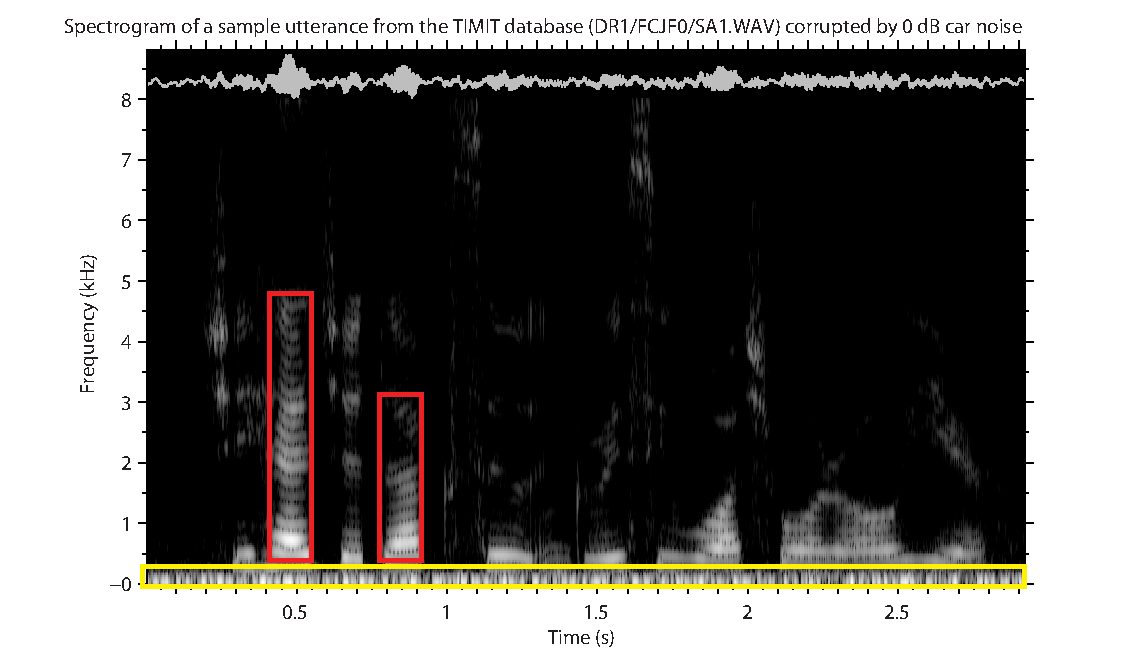
\includegraphics[width=0.9\columnwidth]{Figures/Chapter2/harmospgramcar.pdf}
		\rule{37em}{0.5pt}
	\caption[Spectrogram of a sample utterance corrupted by car noise under 0 dB SNR]{Spectrogram of a sample utterance corrupted by car noise under 0 dB SNR}
	\label{fig:harmospgramcar}
\end{figure}

\begin{figure}[htbp]
	\centering
		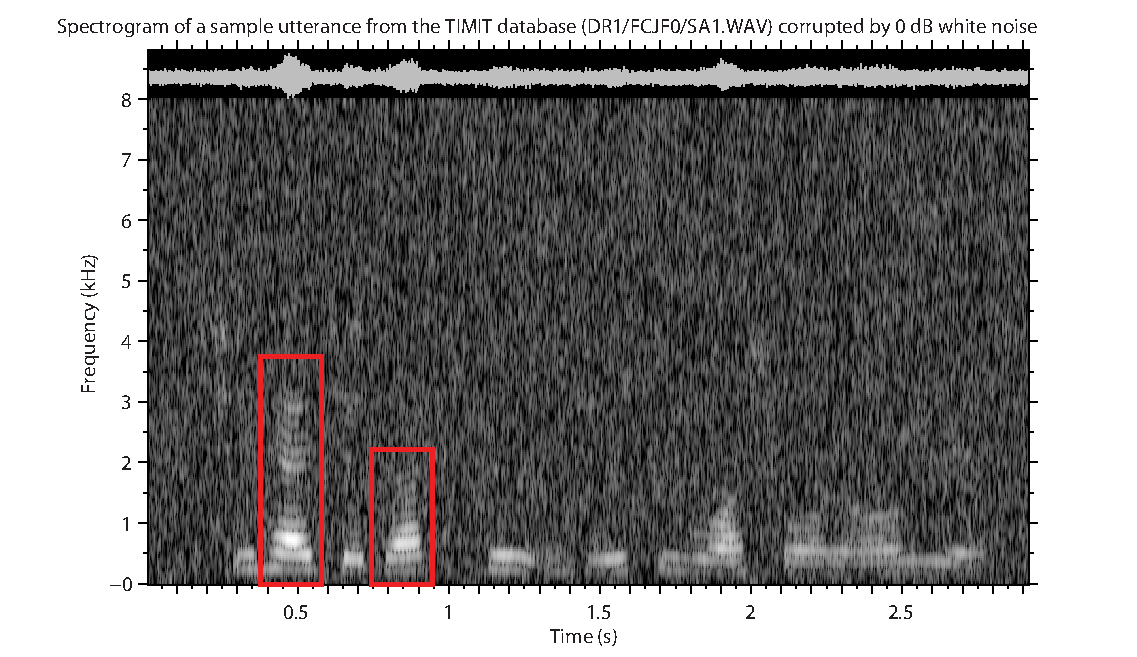
\includegraphics[width=0.9\columnwidth]{Figures/Chapter2/harmospgramwhite.pdf}
		\rule{37em}{0.5pt}
	\caption[Spectrogram of a sample utterance corrupted by white noise under 0 dB SNR]{Spectrogram of a sample utterance corrupted white noise under 0 dB SNR}
	\label{fig:harmospgramwhite}
\end{figure}

In \cite{PARADE} Ishizuka \emph{et al.} proposed a VAD (dubbed PARADE) based on the ratio of the powers of periodic to aperiodic components of the signal. A block diagram of the algorithm is presented in \ref{fig:PARADE}. The VAD decision is based on the likelihood ratio defined in Equation \ref{eq:PARADE} where $\phi (i)$ equals $\frac{\hat{\lambda}_p (i)}{\hat{\lambda}_a (i)}$ - the ratio of the average power per frequency bin of the periodic to aperiodic components of the signal in frame $i$.

\begin{equation}
\Lambda(i) = \frac{1}{\phi (i)} \exp \left\{ \frac{1}{2} \left( \phi (i)^{2} - \frac{1}{\phi (i)^{2}} \right) \right\}
\label{eq:PARADE}
\end{equation}

The authors propose to approximate the average powers from Equations \ref{eq:aperiodicpower} and \ref{eq:periodicpower} where $\vartheta$ is the number of harmonics in the current frame and $\eta$ is a specific constant for power estimation.

\begin{equation}
\hat{\lambda}_a = \frac{\lambda - \eta \sum_{m=1}^{\vartheta} \left| X(m f_0) \right|^{2}}{1-\eta \vartheta}
\label{eq:aperiodicpower}
\end{equation}

\begin{equation}
\hat{\lambda}_p = \lambda - \hat{\lambda}_a
\label{eq:periodicpower}
\end{equation}

\begin{figure}[htbp]
	\centering
		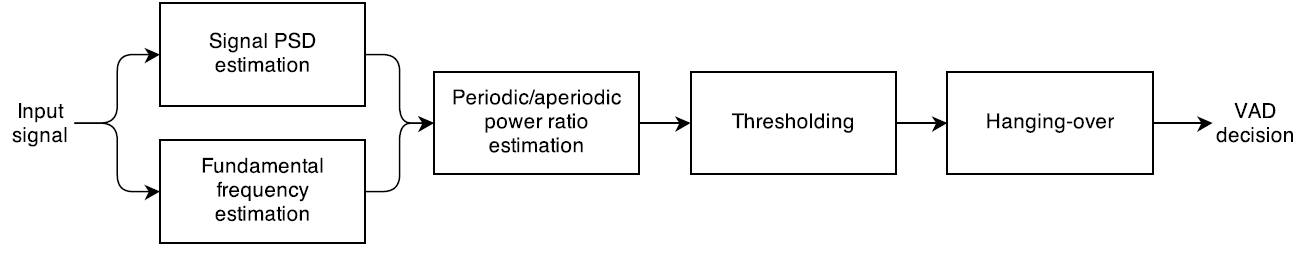
\includegraphics[width=0.9\columnwidth]{Figures/Chapter2/PARADE.png}
		\rule{37em}{0.5pt}
	\caption[Block diagram of the periodic/aperiodoc component ratio VAD]{Block diagram of the periodic/aperiodoc component ratio VAD \cite{PARADE}}
	\label{fig:PARADE}
\end{figure}

While this concept is likely to be robust to various non-stationary noise types, by definition it cannot cope with the unvoiced parts of speech, detection of which has to be performed by a hang-over scheme. In the original paper, the authors did not specify how to estimate the number of harmonics $\vartheta$ for each frame, which is crucial to the proper working of the algorithm. A potential improvement might also come from an improved pitch detection method.

Another approach to using harmonic frequency components\footnote{This algorithm also builds on the idea of LRT described in section \ref{ssec:LRT}. The main improvement comes however from utilising the spectral harmonicity therefore it has been included in this section} for VAD has been investigated by Tan \emph{et al.} in \cite{Tan}. The authors claim, that under low SNR the approach from \cite{RamirezMulti} is likely to fail since the LRs from the high-energy frames will not be strong enough to aid the proper classification of the low-energy frames. Therefore, they propose a new way of calculating the LRs for the voiced frames, defined in Equation \ref{eq:harmfreq} where $\vartheta$ is the number of harmonics within the resolution of the DFT and $f_0$ denotes the fundamental frequency. The algorithm calculates the LR only using the frequency bins which are multiples of the fundamental frequency.

\begin{equation}
\log \Lambda_v = \frac{1}{\vartheta} \sum_{m=1}^{\vartheta} \log \Lambda(m f_0)
\label{eq:harmfreq}
\end{equation}

Voiced frames are pre-identified by the pitch determination algorithm, and all others are considered as unvoiced. The LR for the unvoiced frames is calculated in a standard way from \cite{SohnInitial} i.e. by considering all frequency bins.

\subsection{Summary}

Voice Activity Detection has been studied by numerous researchers over the recent years. Some of the most simple features proposed in the literature, apart from energy, are based on the entropy of the signal, either in time or frequency domain.

The popular LRT based approach, initially proposed by Sohn \emph{et al.}, has served as a basis for many researchers who tried to improve the original algorithm. While Sohn \emph{et al.} employed the LRT to the SNR, the idea has also been applied to other features, such as the periodic to aperiodic component ratio. Nevertheless, many VAD algorithms still utilise the estimated SNR as a voicing feature. Ramirez \emph{et al.} proposed one such VAD, where the SNR is calculated for a given frame including information from the neighbouring frames, rather than considering each frame independently.

The most noise-robust VAD algorithms are likely to be the ones which are based on the harmonicity of the speech signal. Since voiced speech typically does not present high energy in all frequency bins, it is beneficial to first identify the fundamental frequency of a signal and consider the power around the multiples of it. While this approach inherently cannot detect the aperiodic unvoiced phonemes, a clever hang-over scheme can help in their proper classification by extending the initial VAD decisions to include such misdetected speech segments.

%----------------------------------------------------------------------------------------
%	SECTION 3 - Conclusion
%----------------------------------------------------------------------------------------

\section{Conclusion}

This chapter presented a literature survey of the most commonly encountered approaches to Voice Activity Detection. In section \ref{sec:StandardVADs} some standard algorithms have been described while section \ref{sec:RobustVADs} reviewed the recent research efforts in the VAD area.

In terms of noise-robustness, the standard algorithms are unlikely to achieve satisfactory performance under low SNR conditions since they are primarily based on features such as the energy or the zero-crossing rate which are easily degradable by high background noise levels. In such conditions, performance of the recently proposed VAD algorithms is expected to be much better. 
%% Chapter Template

\chapter{Experimental set-up} % Main chapter title

\label{Chapter3} % Change X to a consecutive number; for referencing this chapter elsewhere, use \ref{ChapterX}

\lhead{Chapter 3. \emph{Experimental set-up}} % Change X to a consecutive number; this is for the header on each page - perhaps a shortened title

%--------------------------------------------------------
%	SECTION 1 - Motivation
%--------------------------------------------------------

\section{Motivation}

A large number of VAD algorithms proposed in the literature, the lack of standard methods for their evaluation and an abundance of speech and noise corpora makes it difficult to compare the results reported in the research papers. Therefore, the identification of an algorithm whose performance is objectively best is not possible without their proper benchmarking. In fact, it can be hypothesised that such objectively best algorithm does not exist since the performance of the algorithms will, at least to some extent, depend on the specific application and the encountered noise type. Another problem emerges from a variety of different hang-over schemes used in the experiments from the literature. These schemes can greatly affect the final VAD decisions and their use is especially important with the harmonicity based features which rely exclusively on the hang-over scheme for the detection of unvoiced phonemes. In order to unify the effect of hanging-over, the same scheme should be applied to all VAD features. Finally, some algorithms require estimation of the same values before the actual decision feature can be computed. For the algorithms chosen in this evaluation, these include noise power spectrum and pitch estimation. In order to reduce the performance bias coming from these estimates, the same procedures should be applied to all algorithms.

Therefore, the first aim of this chapter is to describe the implementation details of the selected VAD algorithms so that the differences in their operation can be easily identified\footnote{Ideally, they should differ only in the voicing features used for classification.}. Secondly, the speech and noise recordings as well as the corresponding procedure for obtaining the ground truth labels (for speech/non-speech) are presented so that the experiments can be repeated. For speech, a subset of the TIMIT \cite{TIMIT} database has been used. Recordings of various noise types have been taken from the NOISEX-92 \cite{NOISEX} database and added to the clean speech at various power levels.

%--------------------------------------------------------
%	SECTION 2 - VAD features
%--------------------------------------------------------

\section{VAD features}

Due to a large number of VAD features proposed in the literature, implementation and evaluation of all of them is impractical. However, a small number of features which appear to be noise-robust, based on different ideas and, ideally, recently published can be selected for comparison. In this evaluation, the features from the following VAD algorithms have been implemented:

\begin{itemize}
\item A Statistical Model-Based Voice Activity Detector \cite{Sohn} (hereinafter referred to as `Sohn')
\item Efficient Voice Activity Detection Algorithms Using Long-term Speech Information \cite{LTSD} (hereinafter referred to as `LTSD')
\item Entropy Based Voice Activity Detection in Very Noisy Conditions \citep{Renevey} (hereinafter referred to as `Entropy')
\item Noise Robust Voice Activity Detection Based on Periodic to Aperiodic Component Ratio \cite{PARADE} (hereinafter referred to as `PARADE')
\item Voice Activity Detection using Harmonic Frequency Components in Likelihood Ratio Test \cite{Tan} (hereinafter referred to as `Harmfreq')
\end{itemize}

In particular, the LTSD feature has been chosen because it is calculated taking into account multiple frames surrounding the one for which the decision is being made. Harmfreq is similar the Sohn feature, but calculates the likelihood ratio for the voiced phonemes only at the multiples of the fundamental frequency, hence it is a mixture of a LRT algorithm and a harmonicity based one. PARADE, on the other hand, is supposed to be robust to a variety of non-stationary noise types.

\subsection{Shared implementation parts}

The calculation of a number of VAD features requires prior estimation of some signal characteristics. In particular, Sohn, LTSD and Harmfreq need a noise power spectrum for the SNR estimate. Similarly, PARADE and Harmfreq require a pitch estimate in order to calculate the power of the signal at its multiples. In the original research papers either no procedure has been recommended (i.e. in Sohn \cite{Sohn} for noise PSD estimation) or different procedures have been suggested for estimation of the same property (i.e. pitch estimation in PARADE \cite{PARADE} and Harmfreq \cite{Tan}). In order to reduce the bias coming from potentially different estimation procedures, the same noise and pitch estimation algorithms have been applied to all VAD features. For the noise PSD, an implementation of the MMSE noise power estimator \cite{MMSEnoise} provided by VOICEBOX \cite{VOICEBOX} has been used. Similarly, the fundamental frequency in PARADE and Harmfreq has been estimated using PEFAC \cite{PEFAC}. Finally, before any processing, the incoming speech signal has been divided into 50 ms-long non-overlapping frames and windowed with a periodic Hanning window.

\subsection{Algorithm-specific implementation parts}

Apart from the same implementation parts used by different algorithms, there are parameters which are specific to some VAD features. Summary of the algorithm-specific implementation details is presented below:

\begin{itemize}
\item Sohn - the constant for decision-directed a priori SNR estimation is $\alpha = 0.95$
\item LTSD - the LTSE lookup into neighbouring frames is $N = 3$. Note that it is a smaller value than $N=6$ recommended in \cite{LTSD} due to a longer frame length and a lack of the overlap factor
\item PARADE - the number of harmonics is $\vartheta = 10$ or the maximum that fit in the resolution of the DFT
\item Harmfreq - $\alpha = 0.95$ (same as in Sohn). $\vartheta = 10$ or the maximum that fit in the resolution of the DFT (same as in PARADE). A frame is treated as voiced if the probability returned by PEFAC is greater than $0.5$
\end{itemize}

%--------------------------------------------------------
%	SECTION 3 - Hang-over scheme
%--------------------------------------------------------

\section{Hang-over scheme}
\label{sec:hang}

In order to reduce the differences in the final VAD decisions coming from different hang-over schemes, the same method has been applied to all evaluated VAD features, pseudo code of which is presented in Algorithm \ref{algo:hangover}. This is a modified and adapted to the chosen frame length version of the scheme originally published by ETSI in \cite{ETSIHangover}. This particular algorithm has been chosen because of its simplicity and good results achieved in the evaluation.

The main idea behind the scheme is to initialise the so-called \emph{hang-over timer} whenever the maximum number of consecutive speech decisions in the look-ahead buffer of $B$ frames is greater than $S_p$ (speech possible) or $S_l$ (speech likely). The proposed value for $B$ by ETSI is $7$ and the same has been used in this implementation. However, the values for parameters $S_p$, $S_l$, $L_s$ and $L_m$ were made smaller than the ones outlined in the standard, since the length of the processed signal frames is longer (i.e. 50 ms) and there is no overlap between them.

\begin{algorithm}
\textbf{INPUT:} $F$ - number of frames \\
\textbf{INPUT:} $V$ - VAD decisions prior to the hang-over scheme \\
\textbf{OUTPUT:} $hV$ - VAD decisions after the hang-over scheme
\begin{algorithmic}[1]
\STATE $B \leftarrow 7$ \COMMENT{buffer length}
\STATE $S_p \leftarrow 2$ \COMMENT{speech possible} 
\STATE $S_l \leftarrow 3$ \COMMENT{speech likely}
\STATE $L_s \leftarrow 5$ \COMMENT{short hang-over time}
\STATE $L_m \leftarrow 8$ \COMMENT{medium hang-over time}
\STATE
\STATE $T \leftarrow 0$ \COMMENT{hang-over timer}

\FOR{$i=1$ to $F-B+1$}
\STATE $CB \leftarrow V(i:i+B-1)$ \COMMENT{current buffer of VAD decisions}
\STATE $M \leftarrow$ maximum consecutive speech-present decisions in $CB$
\IF{$M \geqslant S_l$}
\STATE $T \leftarrow L_m$
\ELSIF{$M \geqslant S_p$ \AND $T < L_s$}
\STATE $T = L_s$
\ELSIF{$M < S_p$ \AND $T > 0$}
\STATE $T \leftarrow T-1$
\ENDIF
\IF{$T > 0$}
\STATE $hV(i) \leftarrow 1$
\ELSE
\STATE $hV(i) \leftarrow 0$
\ENDIF
\ENDFOR
\STATE $hV(F-B+2:F) \leftarrow V(F-B+2:F)$ \COMMENT{assign the pre hang-over decisions to the last B-1 frames}
\RETURN $hV$
\end{algorithmic}
\caption{Hang-over scheme used in all VAD algorithms}
\label{algo:hangover}
\end{algorithm}

%--------------------------------------------------------
%	SECTION 4 - Speech corpus
%--------------------------------------------------------

\section{Speech corpus}

There exists a number of speech corpora for evaluation of VAD and ASR. The choice of a specific corpus is a subjective matter and a large number of them have been used in the literature, making the results reported by the researchers not directly comparable. For the English language the TIMIT speech corpus \cite{TIMIT} seems to be the most widely used and hence has been selected as a source of utterances for this evaluation. There are a number of issues with the original recordings which need to be resolved so that the evaluation can be more accurate. These are:

\begin{itemize}
\item Single utterances are on average no longer than 4 seconds and hence too short for a proper VAD evaluation
\item The recordings contain a very small number of non-speech segments
\item There are differences in the average power between the utterances
\end{itemize}

In order to deal with the first two issues, a number of randomly chosen utterances from every dialect (i.e. DR1 to DR8) has been concatenated into a single speech recording, adding 2.5 seconds of silence at the beginning, ending and between the utterances. In an attempt to equalise the power, the amplitude of each utterance has been normalised such that the average power per sample of all of them is equal. This is important because if the concatenated utterances differed in the average power level, after adding the noise, the one with initially higher power could be easily detected by almost any VAD procedure while the detection of the other one would be very difficult due to the much lower segmental/short-time SNR.

For a proper VAD evaluation, the ground truth speech/non-speech labels need to be obtained. While this might seem like a simple task, it actually includes a degree of subjectivity. Consider Figure \ref{fig:groundtruth} where the speaker first makes a short pause between words and then, after the utterance, takes a breath while still standing near the microphone. Whether the first segment should be classified as speech, since it clearly forms a part of a longer utterance, or silence, since if considered in isolation, it does not exhibit any obvious speech characteristics, is a matter of choice. In this work, all such segments and alike have been treated as integral parts of the utterances and hence classified as speech in the ground truth labels. Obviously, the breath part is not speech and should be treated as such. The initial labels have been obtained by a simple energy VAD and examined visually, making necessary manual changes to any obviously misclassified segments, taking into account the decisions described before.

\begin{figure}[htbp]
	\centering
		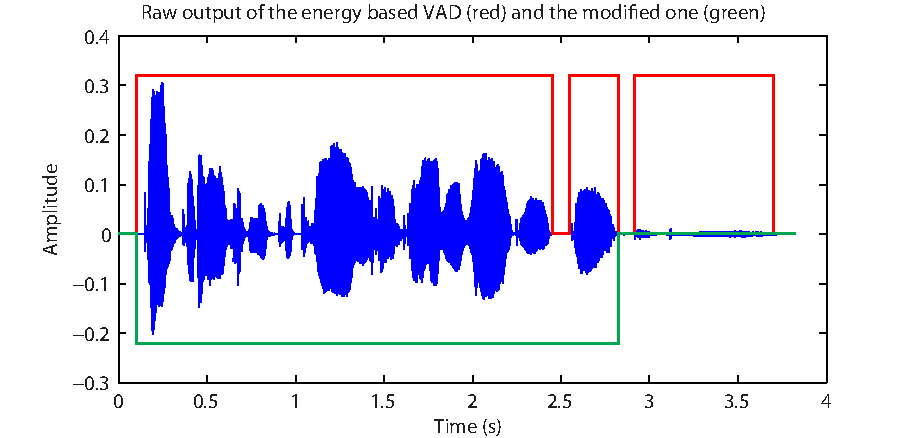
\includegraphics[width=1.0\columnwidth]{Figures/Chapter3/groundtruthbold.pdf}
		\rule{37em}{0.5pt}
	\caption[Raw and modified outputs from the energy based VAD used as ground truth labels]{Raw and modified outputs from the energy based VAD used as ground truth labels}
	\label{fig:groundtruth}
\end{figure}

%--------------------------------------------------------
%	SECTION 5 - Noise corpus and SNR
%--------------------------------------------------------

\section{Noise corpus and SNR}

Similarly to the speech corpora, there exists a large number of noise databases which are commonly used for evaluation of speech processing algorithms. In this evaluation, most noise types have been taken from the NOISEX-92 \cite{NOISEX} corpus with the exception of the babble noise which has been adapted from the Nato Noise \cite{Nato} package. Also, the white noise has been generated\footnote{The white noise has been generated only once. The exact same samples have been used for evaluation of all algorithms.} by MATLAB's \texttt{randn} function which returns samples of the naturally distributed Gaussian random variable with zero mean\footnote{In this case, the variance, which by default is 1, is irrelevant since the noise is scaled before addition to the clean speech signal anyway.}. The complete list of the noise types used in this evaluation is: white, car, spchspect, babble, opsroom and factory.

In order to evaluate the algorithms' performance under different conditions, the clean speech and noise signals need to be scaled to the desired SNR. This is achieved by the following procedure which ensures the correct power of noise relative to the speech:

\begin{enumerate}
\item Calculate the active level of the clean speech signal\footnote{The active level of a speech signal is defined to be its average power during intervals when speech is present.} $P_s$
\item Calculate the average power of noise $P_n$
\item Calculate the scaling constant for noise as $\sqrt{\frac{P_s}{10^{\text{SNR}/10} \times P_n}}$
\item Multiply each noise sample by the scaling constant
\item Add the scaled noise signal to the clean speech signal
\end{enumerate}

%--------------------------------------------------------
%	SECTION 6 - Summary
%--------------------------------------------------------

\section{Summary}

This chapter described the important considerations and choices which have been made with respect to the experimental set-up. An effort has been made to unify as many of the algorithm's parts as possible so that the actual voice detection features can be compared objectively. All algorithms will be evaluated on the same speech and noise recordings under various SNRs. Finally, the same hang-over scheme will be applied to all features in order to remove the variance in the results coming from the performance of different schemes as opposed to the quality of the voice detection features.
%% Chapter Template

\chapter{Evaluation of VAD algorithms} % Main chapter title

\label{Chapter4} % Change X to a consecutive number; for referencing this chapter elsewhere, use \ref{ChapterX}

\lhead{Chapter 4. \emph{Evaluation of VAD algorithms}} % Change X to a consecutive number; this is for the header on each page - perhaps a shortened title

%------------------------------------------------
%	SECTION 1 - Evaluation methods
%------------------------------------------------

\section{Evaluation methods}

Voice Activity Detection is a binary classification problem in which each frame of the incoming signal can only be classified as speech or non-speech. For such types of problems, a number of standard evaluation methods exist. Most of them revolve around different ratios of the four fundamental quantities which are calculated by comparing the outcome of an experiment and the so-called \emph{gold standard/ground truth} which is the best guess of the true classification. In terms of VAD, these are:

\begin{itemize}
\item True Positive (TP) - speech classified correctly
\item True Negative (TN) - non-speech classified correctly
\item False Positive (FP) - non-speech classified incorrectly
\item False Negative (FN) - speech classified incorrectly
\end{itemize}

Some of the most popular ratios are:
\begin{itemize}
\item Precision (aka positive predictive value) = $\frac{\text{TP}}{\text{TP}+\text{FP}}$
\item Specificity (aka true negative rate) = $\frac{\text{TN}}{\text{TN}+\text{FP}}$
\item Recall (aka sensitivity or true positive rate) = $\frac{\text{TP}}{\text{TP}+\text{FN}}$
\item Fall-out (aka false positive rate) = $\frac{\text{FP}}{\text{TN}+\text{FP}}$ = (1-specificity)
\item Accuracy = $\frac{\text{TP}+\text{TN}}{\text{TP}+\text{FP}+\text{TN}+\text{FN}}$
\end{itemize}

\subsection{Receiver Operating Characteristic curves}

At the beginning of the classification stage most VAD algorithms use a threshold. If the feature value calculated for the current frame is above it (or below in some algorithms) then this signal segment is classified as speech and non-speech otherwise. Therefore, the number of frames classified as speech/non-speech varies greatly with the value of the threshold. Setting a very low value can result in all processed frames being classified as speech, yielding 100\% recall but also 0\% specificity. Conversely, setting a very high threshold might result in very good specificity but bad recall. Needless to say that the extreme values of the threshold result in an useless algorithm.

In order to capture the trade-off between the true and false positive rates, the so-called Receiver Operating Characteristic (ROC) curves have been created, an example of which is presented in Figure \ref{fig:roc}. The blue line can be interpreted as a performance of a completely random classifier. The green curve represents a much better performance while the red one much worse. Perfect classification is obtained in the (0,1) point i.e. 100\% recall (no false negatives) and 100\% specificity (no false positives). An average performance of the VAD algorithm across all values of the threshold can be compactly described by calculating the Area Under Curve (AUC) which, as the name implies, is the area under the ROC curve with the best possible value of 1.

\begin{figure}[htbp]
	\centering
		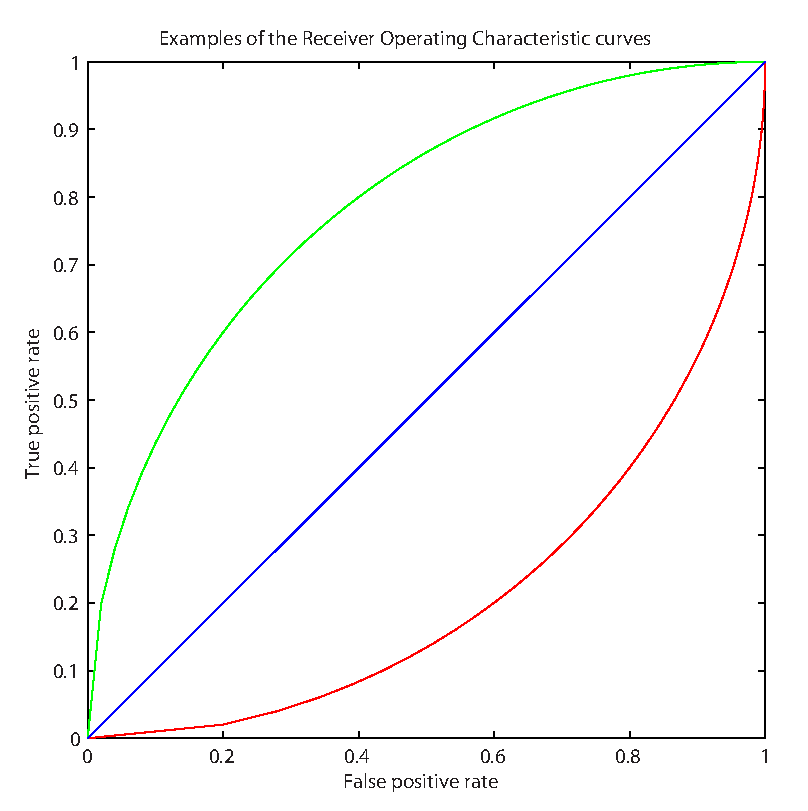
\includegraphics[width=0.55\columnwidth]{Figures/Chapter4/roc.pdf}
		\rule{37em}{0.5pt}
	\caption[Examples of the Receiver Operating Characteristic curves]{Examples of the Receiver Operating Characteristic curves}
	\label{fig:roc}
\end{figure}

\subsection{Speech/non-speech hit rates}

While the ROC curves capture the performance of a VAD algorithm across different thresholds, in practise, a single, fixed value is often chosen. This fact can have quite severe implications on algorithms whose best performance, captured by the ROC curve under many noise types and SNRs, exists at different thresholds. An algorithm cannot be called truly robust if it requires tweaking in its parameters to perform satisfactorily in various conditions. Therefore it is also important to evaluate the algorithms' performance with a single threshold value. Such evaluation can be carried out by plotting the so called \emph{speech hit-rate} (i.e. recall) and \emph{non-speech hit rate} (i.e. specificity) when the algorithms are implemented with a fixed threshold value, selected by examination of the ROC curves in different conditions. In this evaluation, the \emph{optimal} threshold has been identified by selecting the points on the ROC curves where the TPR and FPR are closest to being equal (in -5 and 0 dB SNRs) and calculating the mean of the corresponding threshold values while discarding the 2 most extreme ones.

%----------------------------------------------------------------------
%	SECTION 2 - Evaluation results
%----------------------------------------------------------------------

\section{Evaluation results}

In the two experiments, the selected VAD algorithms have been implemented and evaluated with and without the hang-over scheme described in Section \ref{sec:hang}. The ROC curves have been plotted for all six noise types at two low SNRs i.e. -5 dB and 0 dB. In order to capture the average performance, the AUC values have also been calculated. Finally, the most promising threshold for each algorithm across the two low SNRs and six noise types has been identified and the speech/non-speech hit rates at six different SNRs (20 dB to -5 dB) have been calculated.

In this chapter, only the results under two lowest SNRs (-5 dB and 0 dB) are going to be presented. Additional evaluation results for other SNRs have been put in Appendix \ref{AppendixA}.

\subsection{VAD algorithms with hang-over}

Figures \ref{fig:-5dBh} and \ref{fig:0dBh} present the ROC curves for all evaluated algorithms with hang-over for the six types of noise under -5 dB and 0 dB SNR respectively. In almost all cases, the LTSD algorithm (red line) seems to outperform all other VAD methods under both SNRs. In car noise, its performance is a bit worse than both the Sohn and Harmfreq's algorithms however it should be noticed that most algorithms perform exceptionally well in this type of noise. This can be explained by the fact that car noise occupies predominantly the low frequencies and the estimation procedure is able to track the noise well enough even at negative SNR. In factory noise, all algorithms seem to exhibit performance close to a random guess since all ROC curves are close to the 45$^\circ$ line.

The best average performance of the LTSD algorithm is confirmed by examination of the AUC values under -5 dB SNR presented in Table \ref{tab:AUC-5dBh} where the best value for the given noise type is highlighted in green while the worst one in red. The LTSD VAD outperforms all other algorithms in 4 out of 6 cases which results in the best average performance. On the other hand, the Entropy VAD is the worst performing algorithm in 5 out of 6 cases.

\begin{table}[htbp]
\center
\begin{tabular}{c|c|c|c|c|c|c!{\vrule width 1.5pt}c|}
\cline{2-8}
 & white & car & spchspect & babble & opsroom & factory & average \\ \hline
\multicolumn{1}{ |c| }{Sohn} & 0.8561 & 0.9595 & 0.9063 & 0.7786 & 0.8276 & 0.5671 & 0.8159\\ \hline
\multicolumn{1}{ |c| }{LTSD} & \textcolor{LimeGreen}{0.9497} & 0.9496 & \textcolor{LimeGreen}{0.9502} & \textcolor{LimeGreen}{0.8842} & \textcolor{LimeGreen}{0.8586} & 0.6345 & \textcolor{LimeGreen}{\textbf{0.8711}}\\ \hline
\multicolumn{1}{ |c| }{Entropy} & 0.9160 & \textcolor{red}{0.4999} & \textcolor{red}{0.5807} & \textcolor{red}{0.4832} & \textcolor{red}{0.4350} & \textcolor{red}{0.5315} & \textcolor{red}{\textbf{0.5744}}\\ \hline
\multicolumn{1}{ |c| }{PARADE} & \textcolor{red}{0.9117} & 0.8853 & 0.6159 & 0.5389 & 0.6339 & \textcolor{LimeGreen}{0.7071} & 0.7154\\ \hline
\multicolumn{1}{ |c| }{Harmfreq} & 0.9209 & \textcolor{LimeGreen}{0.9676} & 0.9126 & 0.7165 & 0.7992 & 0.6425 & 0.8265\\ \hline
\end{tabular}
\caption[AUC values of the evaluated algorithms \emph{with} hang-over under -5 dB SNR]{AUC values of the evaluated VAD algorithms \emph{with} hang-over under -5 dB SNR}
\label{tab:AUC-5dBh}
\end{table}

Finally, the speech/non-speech hit rates for the algorithms with hang-over and a fixed threshold are presented in Figure \ref{fig:snrh}. Again, the LTSD VAD exhibits the best speech detection characteristics, however remains slightly behind Harmfreq for the non-speech detection. It is worth reiterating that there is a trade-off between these two evaluation metrics and, especially for Harmfreq, lowering the threshold by a small value could increase the speech hit-rate while decreasing the non-speech's, bringing its performance close to the LTSD's.

\begin{figure}[htbp]
	\centering
		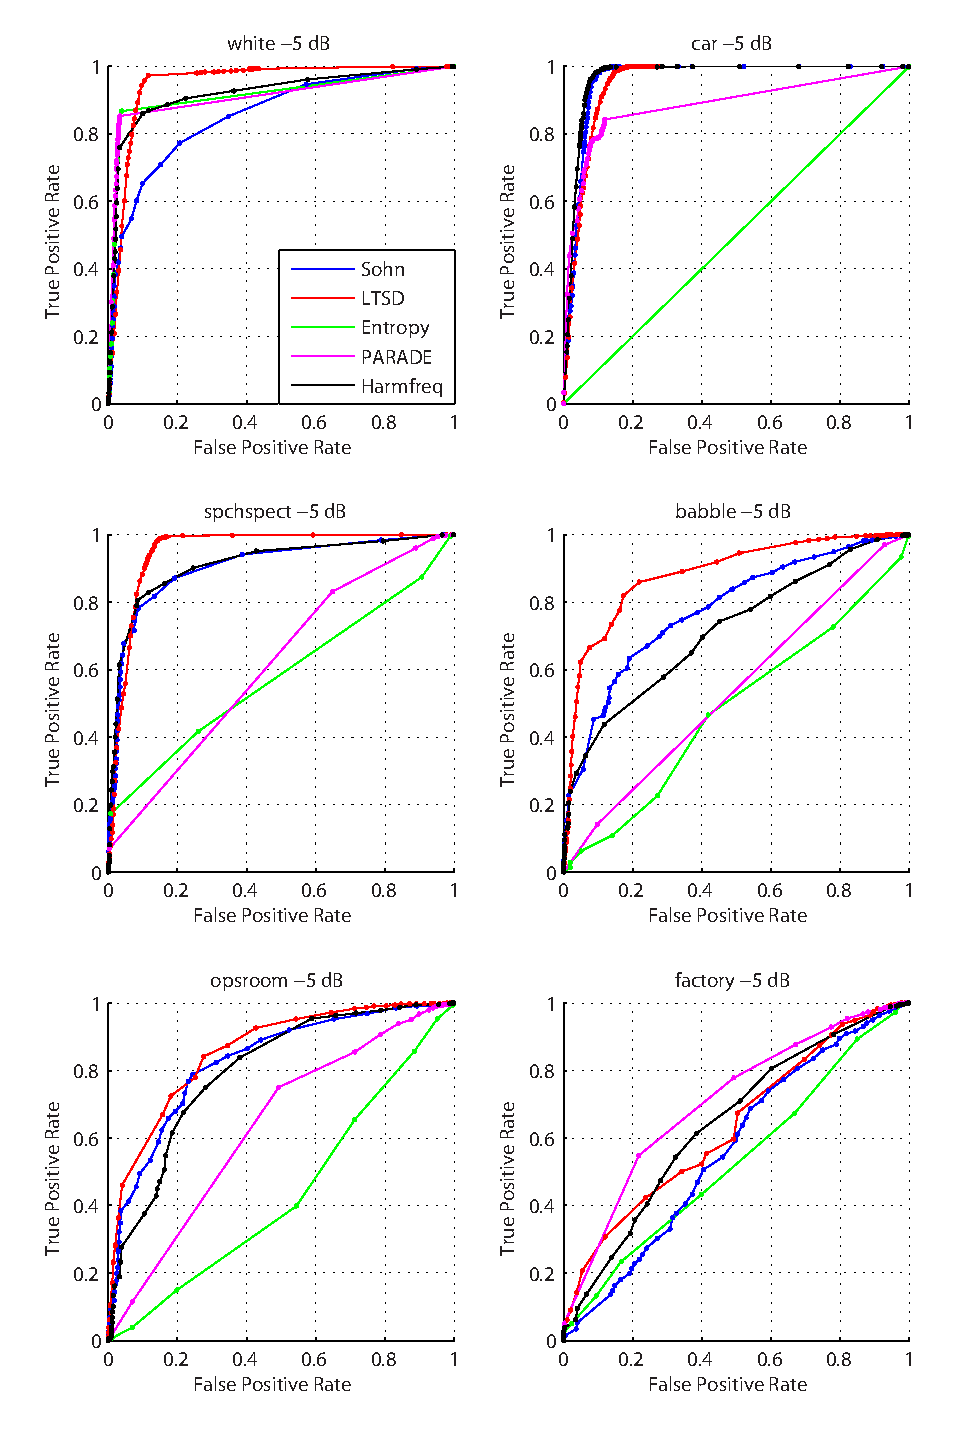
\includegraphics[width=1.0\columnwidth]{Figures/Chapter4/-5dBh.pdf}
		\rule{37em}{0.5pt}
	\caption[ROC curves of the evaluated algorithms \emph{with} hang-over under -5 dB SNR]{ROC curves of the evaluated VAD algorithms \emph{with} hang-over under -5 dB SNR}
	\label{fig:-5dBh}
\end{figure}

\begin{figure}[htbp]
	\centering
		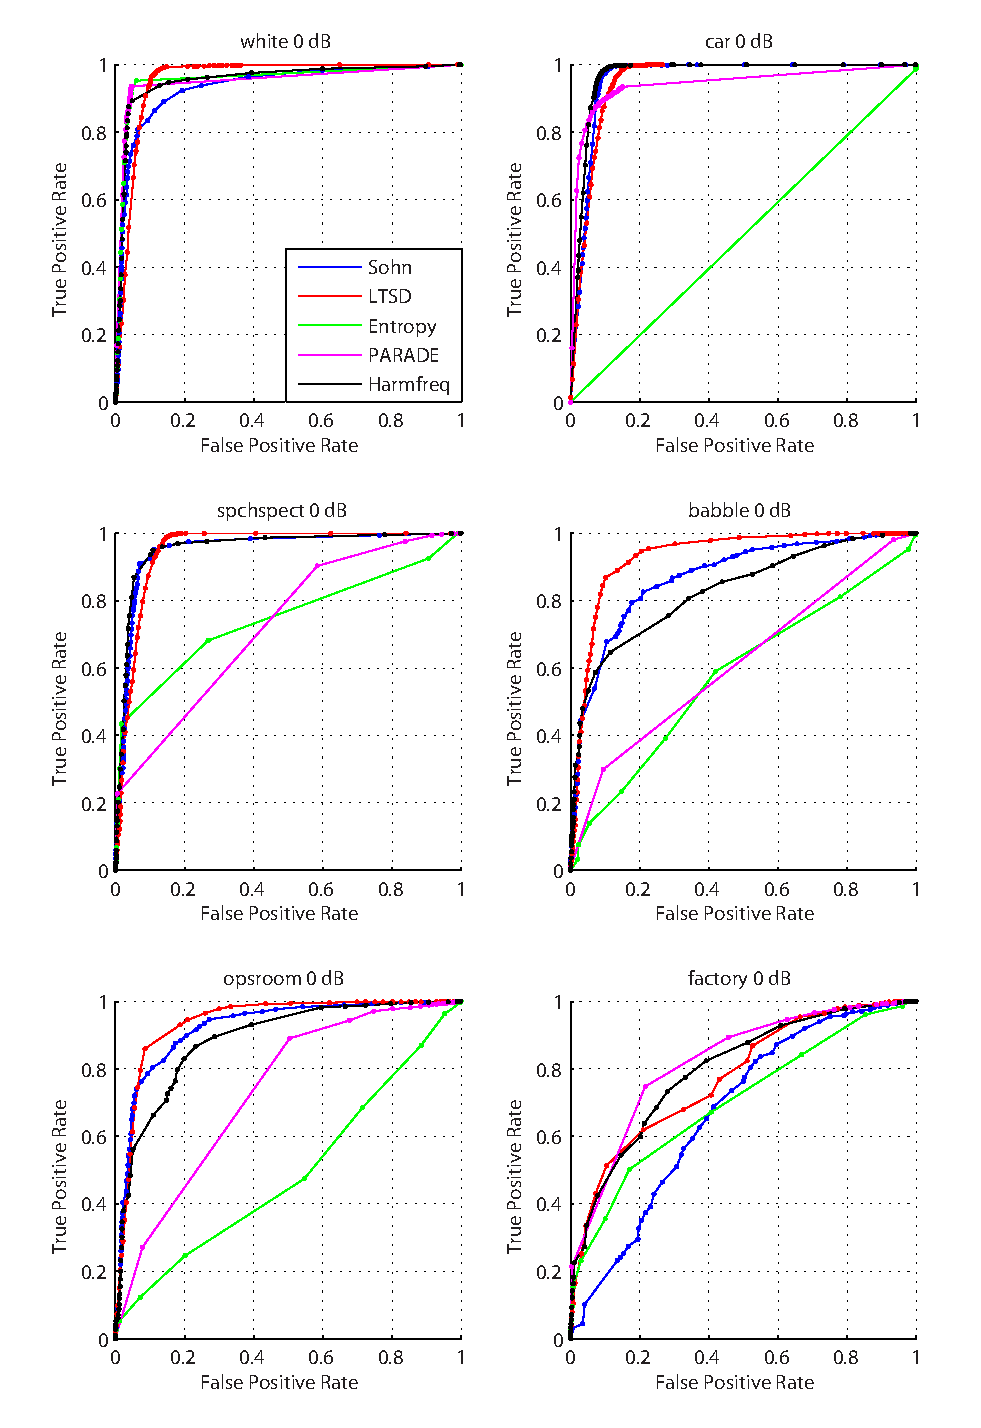
\includegraphics[width=1.0\columnwidth]{Figures/Chapter4/0dBh.pdf}
		\rule{37em}{0.5pt}
	\caption[ROC curves of the evaluated algorithms \emph{with} hang-over under 0 dB SNR]{ROC curves of the evaluated VAD algorithms \emph{with} hang-over under 0 dB SNR}
	\label{fig:0dBh}
\end{figure}

\begin{figure}[htbp]
	\centering
		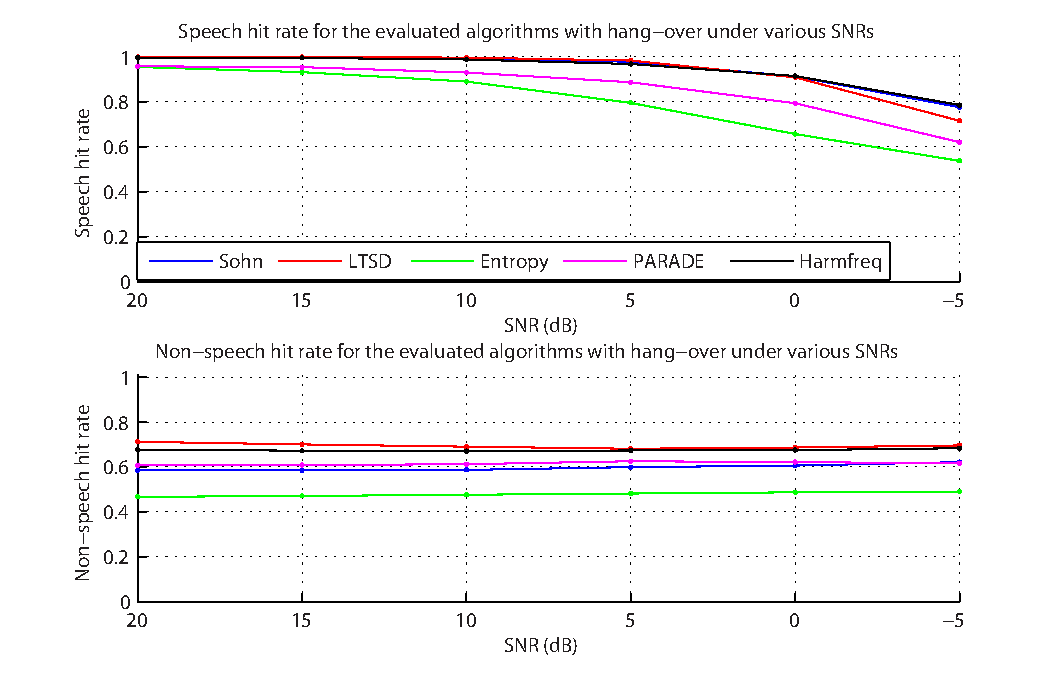
\includegraphics[width=0.9\columnwidth]{Figures/Chapter4/snrh.pdf}
		\rule{37em}{0.5pt}
	\caption[Speech/non-speech hit rates for the evaluated algorithms \emph{with} hang-over under different SNRs]{Speech/non-speech hit rates for the evaluated algorithms \emph{with} hang-over under different SNRs}
	\label{fig:snrh}
\end{figure}

\subsection{VAD algorithms without hang-over}

The same algorithms have also been implemented without the hang-over scheme. It can be argued that this is a more \emph{objective} evaluation of the VAD features since the algorithms stop immediately after the thresholding stage. However, the harmonicity based algorithms are likely to underperform while implemented without the hango-over scheme. Similarly to the previous section, Figures \ref{fig:-5dBnoh} and \ref{fig:0dBnoh} show the ROC curves under -5 dB and 0 dB SNR. Again, the LTSD VAD performs best, while the Entropy VAD exhibits the worst performance. Interestingly, the LTSD's results indicate that the version without hang-over operates better in car noise than the one with. This can be explained by an observation that LTSD without hang-over already achieves such a good performance that when combined with a smoothing scheme, it stretches the speech labels beyond the actual utterances which results in an additional number of false positives.

The best average performance of the LTSD VAD is again confirmed by the AUC values presented in Table \ref{tab:AUC-5dBnoh}. By comparing the two AUC tables (i.e. with and without hang-over) it can be noticed that the LTSD algorithm benefits least from the hang-over scheme. On the other hand, Harmfreq's performance is boosted to the greatest extent. Examination of the speech/non-speech hit rates with a fixed threshold in Figure \ref{fig:snrnoh} again confirms that the LTSD algorithm exhibits the best performance, this time both in the speech as well as in non-speech hit rates.

\begin{figure}[htbp]
	\centering
		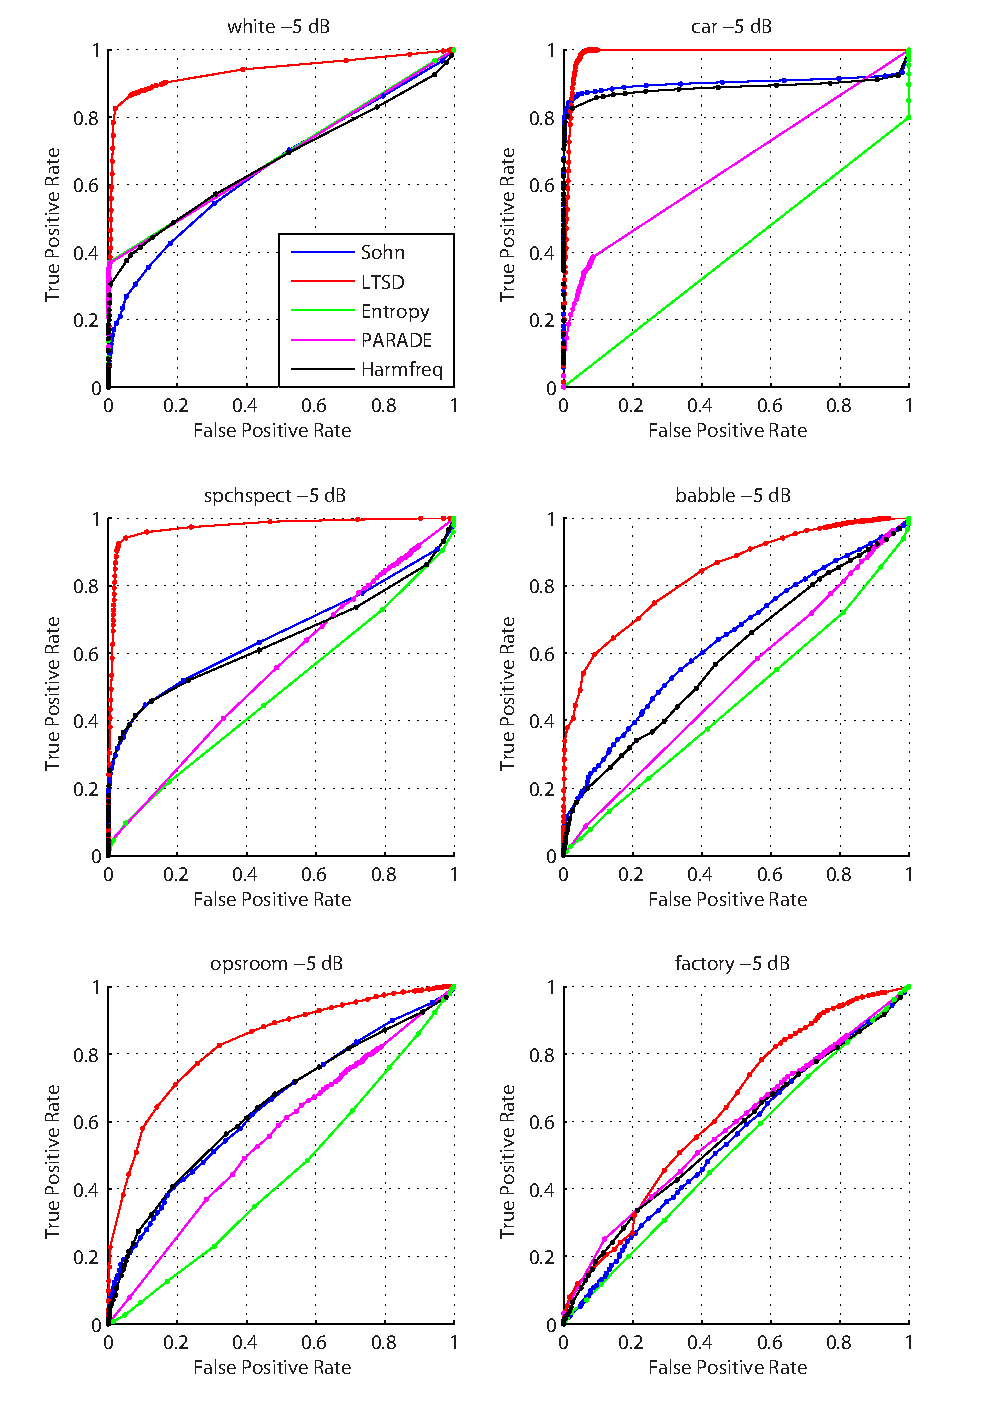
\includegraphics[width=1.0\columnwidth]{Figures/Chapter4/-5dBnoh.pdf}
		\rule{37em}{0.5pt}
	\caption[ROC curves of the evaluated algorithms \emph{without} hang-over under -5 dB SNR]{ROC curves of the evaluated VAD algorithms \emph{without} hang-over under -5 dB SNR}
	\label{fig:-5dBnoh}
\end{figure}

\begin{table}[htbp]
\center
\begin{tabular}{c|c|c|c|c|c|c!{\vrule width 1.5pt}c|}
\cline{2-8}
 & white & car & spchspect & babble & opsroom & factory & average \\ \hline
\multicolumn{1}{ |c| }{Sohn} & 0.6540 & 0.9019 & 0.6564 & 0.6378 & 0.6423 & 0.5424 & 0.6725\\ \hline
\multicolumn{1}{ |c| }{LTSD} & \textcolor{LimeGreen}{0.9365} & 0.9876 & \textcolor{LimeGreen}{0.9741} & \textcolor{LimeGreen}{0.8362} & \textcolor{LimeGreen}{0.8323} & 0.6339 & \textcolor{LimeGreen}{\textbf{0.8668}}\\ \hline
\multicolumn{1}{ |c| }{Entropy} & 0.6856 & \textcolor{red}{0.4007} & \textcolor{red}{0.4878} & \textcolor{red}{0.4561} & \textcolor{red}{0.4425} & \textcolor{red}{0.5160} & \textcolor{red}{\textbf{0.4981}}\\ \hline
\multicolumn{1}{ |c| }{PARADE} & \textcolor{red}{0.6821} & 0.6563 & 0.5514 & 0.5156 & 0.5542 & \textcolor{LimeGreen}{0.5810} & 0.5901\\ \hline
\multicolumn{1}{ |c| }{Harmfreq} & 0.6696 & \textcolor{LimeGreen}{0.8873} & 0.6392 & 0.5912 & 0.6433 & 0.5648 & 0.6659\\ \hline
\end{tabular}
\caption[AUC values of the evaluated algorithms \emph{without} hang-over under -5 dB SNR]{AUC values of the evaluated VAD algorithms \emph{without} hang-over under -5 dB SNR}
\label{tab:AUC-5dBnoh}
\end{table}

\begin{figure}[htbp]
	\centering
		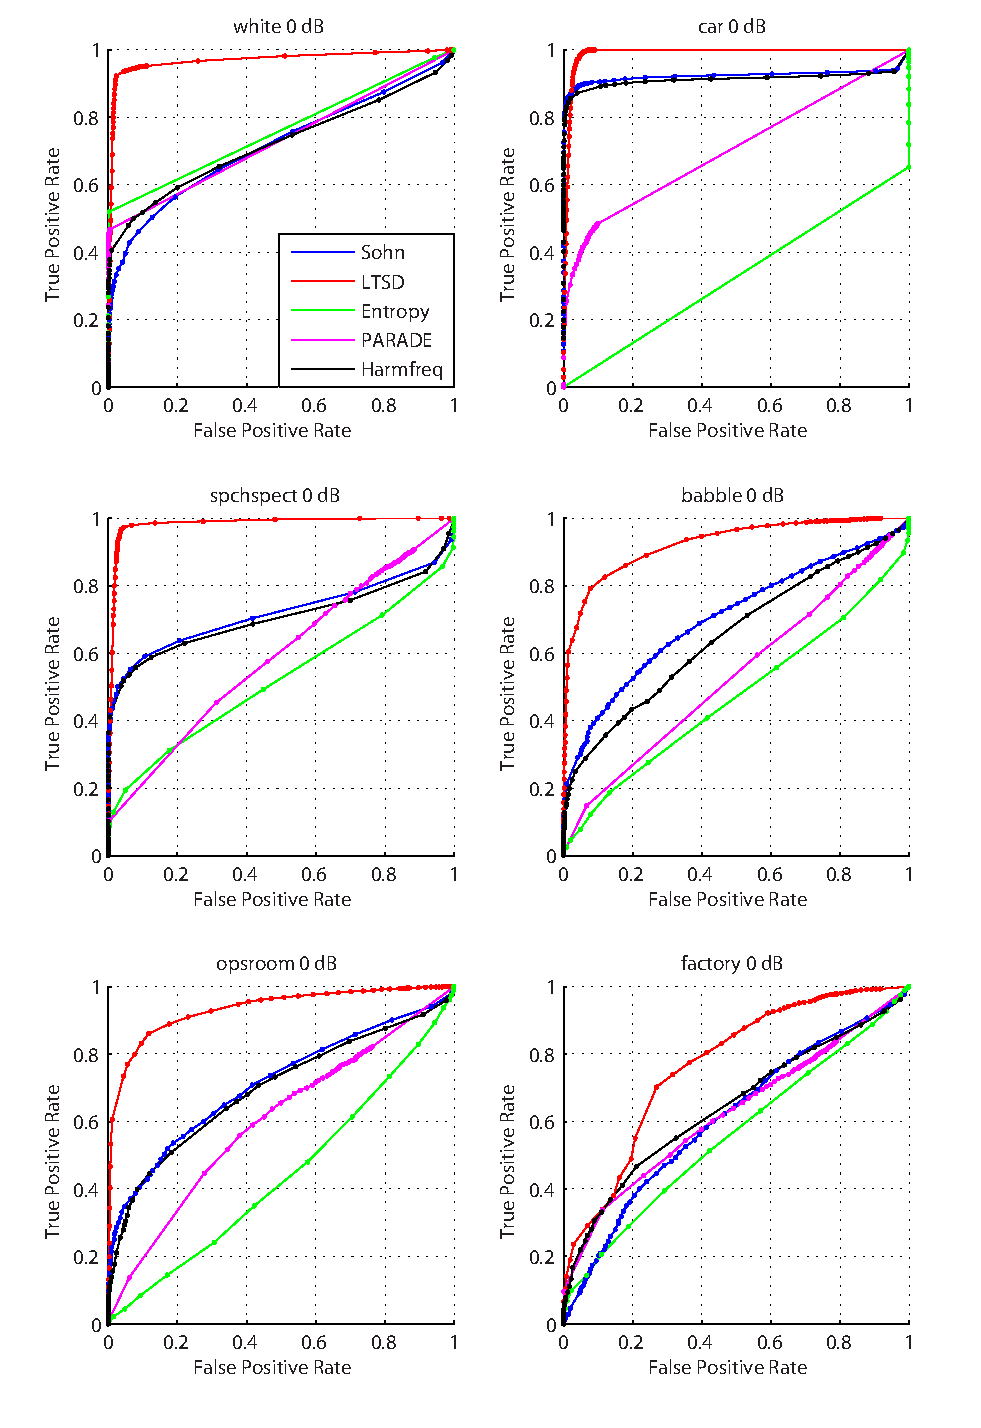
\includegraphics[width=1.0\columnwidth]{Figures/Chapter4/0dBnoh.pdf}
		\rule{37em}{0.5pt}
	\caption[ROC curves of the evaluated algorithms \emph{without} hang-over under 0 dB SNR]{ROC curves of the evaluated VAD algorithms \emph{without} hang-over under 0 dB SNR}
	\label{fig:0dBnoh}
\end{figure}

\begin{figure}[htbp]
	\centering
		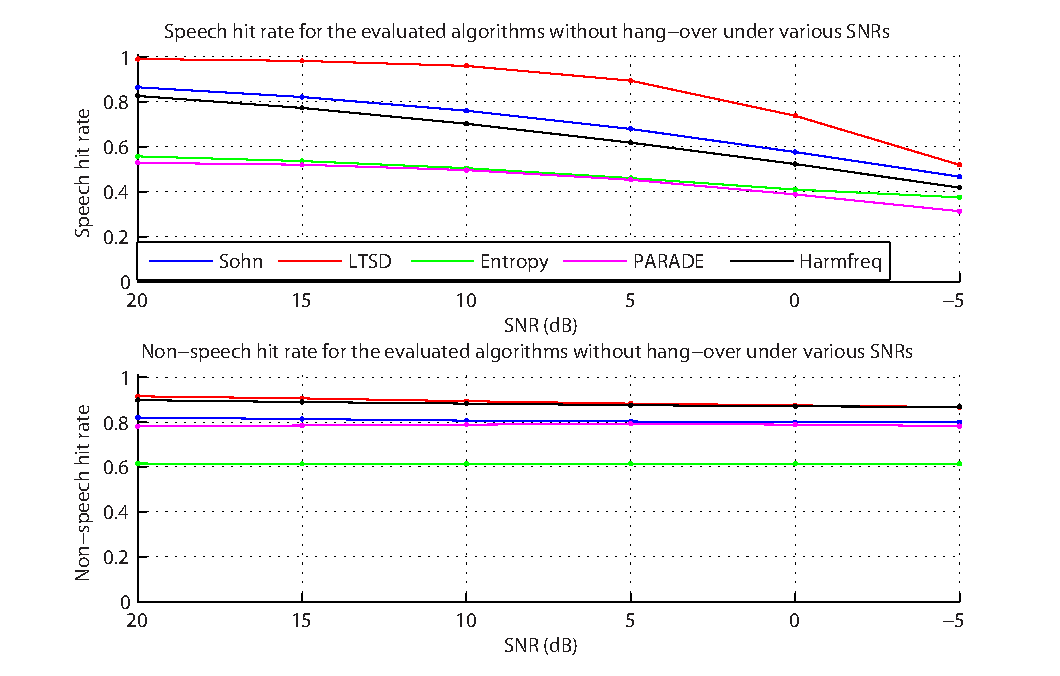
\includegraphics[width=0.9\columnwidth]{Figures/Chapter4/snrnoh.pdf}
		\rule{37em}{0.5pt}
	\caption[Speech/non-speech hit rates for the evaluated algorithms \emph{without} hang-over under different SNRs]{Speech/non-speech hit rates for the evaluated algorithms \emph{without} hang-over under different SNRs}
	\label{fig:snrnoh}
\end{figure}

%----------------------------------------------------------------------
%	SECTION 2 - Conclusion
%----------------------------------------------------------------------

\section{Conclusion}

The evaluation results confirm the hypothesis that the best algorithm cannot be identified for all conditions, which in the real world there is infinitely many of. However, for the evaluated noise types, the LTSD algorithm exhibits the best average performance in 4 out of 6 cases, as concluded from the analysis of Tables \ref{tab:AUC-5dBh} and \ref{tab:AUC-5dBnoh}. Therefore, for practical use, it is beneficial to narrow down the conditions in which the algorithm will have to operate as much as possible. Then, all algorithms can be properly benchmarked and the best one for the specific application could be chosen. Should this be impossible, the best bet is probably to use the LTSD VAD, at least from all the algorithms evaluated in this work. 
%% Chapter Template

\chapter{Conclusion} % Main chapter title

\label{Chapter5} % Change X to a consecutive number; for referencing this chapter elsewhere, use \ref{ChapterX}

\lhead{Chapter 5. \emph{Conclusion}} % Change X to a consecutive number; this is for the header on each page - perhaps a shortened title

%----------------------------------------------------------------------------------------
%	SECTION 1
%----------------------------------------------------------------------------------------

\section{Main Section 1}

Lorem ipsum dolor sit amet, consectetur adipiscing elit. Aliquam ultricies lacinia euismod. Nam tempus risus in dolor rhoncus in interdum enim tincidunt. Donec vel nunc neque. In condimentum ullamcorper quam non consequat. Fusce sagittis tempor feugiat. Fusce magna erat, molestie eu convallis ut, tempus sed arcu. Quisque molestie, ante a tincidunt ullamcorper, sapien enim dignissim lacus, in semper nibh erat lobortis purus. Integer dapibus ligula ac risus convallis pellentesque.

%-----------------------------------
%	SUBSECTION 1
%-----------------------------------
\subsection{Subsection 1}

Nunc posuere quam at lectus tristique eu ultrices augue venenatis. Vestibulum ante ipsum primis in faucibus orci luctus et ultrices posuere cubilia Curae; Aliquam erat volutpat. Vivamus sodales tortor eget quam adipiscing in vulputate ante ullamcorper. Sed eros ante, lacinia et sollicitudin et, aliquam sit amet augue. In hac habitasse platea dictumst.

%-----------------------------------
%	SUBSECTION 2
%-----------------------------------

\subsection{Subsection 2}
Morbi rutrum odio eget arcu adipiscing sodales. Aenean et purus a est pulvinar pellentesque. Cras in elit neque, quis varius elit. Phasellus fringilla, nibh eu tempus venenatis, dolor elit posuere quam, quis adipiscing urna leo nec orci. Sed nec nulla auctor odio aliquet consequat. Ut nec nulla in ante ullamcorper aliquam at sed dolor. Phasellus fermentum magna in augue gravida cursus. Cras sed pretium lorem. Pellentesque eget ornare odio. Proin accumsan, massa viverra cursus pharetra, ipsum nisi lobortis velit, a malesuada dolor lorem eu neque.

%----------------------------------------------------------------------------------------
%	SECTION 2
%----------------------------------------------------------------------------------------

\section{Main Section 2}

Sed ullamcorper quam eu nisl interdum at interdum enim egestas. Aliquam placerat justo sed lectus lobortis ut porta nisl porttitor. Vestibulum mi dolor, lacinia molestie gravida at, tempus vitae ligula. Donec eget quam sapien, in viverra eros. Donec pellentesque justo a massa fringilla non vestibulum metus vestibulum. Vestibulum in orci quis felis tempor lacinia. Vivamus ornare ultrices facilisis. Ut hendrerit volutpat vulputate. Morbi condimentum venenatis augue, id porta ipsum vulputate in. Curabitur luctus tempus justo. Vestibulum risus lectus, adipiscing nec condimentum quis, condimentum nec nisl. Aliquam dictum sagittis velit sed iaculis. Morbi tristique augue sit amet nulla pulvinar id facilisis ligula mollis. Nam elit libero, tincidunt ut aliquam at, molestie in quam. Aenean rhoncus vehicula hendrerit. 
%% Chapter Template

\chapter{Conclusions} % Main chapter title

\label{Chapter6} % Change X to a consecutive number; for referencing this chapter elsewhere, use \ref{ChapterX}

\lhead{Chapter 6. \emph{Conclusions}} % Change X to a consecutive number; this is for the header on each page - perhaps a shortened title

%----------------------------------------------------------------------------------------
%	SECTION 1 - Project outcomes
%----------------------------------------------------------------------------------------

\section{Project outcomes}

The project started with understanding the applications and a general structure of a VAD system (Chapter \ref{Chapter1}). During further literature survey (Chapter \ref{Chapter2}) it became clear that VAD is a very dispersed area of research and a that variety of state-of-the-art algorithms exist. However, identification of the most noise-robust algorithm is difficult as the original performance results are not directly comparable. This motivated the creation of an artificial, yet identical for all algorithms, testing environment (Chapter \ref{Chapter3}) under which a few selected VAD methods could be objectively evaluated (Chapter \ref{Chapter4}). Finally, an approach to adapt one of the recently proposed pitch tracking algorithms to the area of VAD has been undertaken (Chapter \ref{Chapter5}).

While during the evaluation it became clear that the absolutely best VAD algorithm does not exist, as their performance often depends on the noise type and its power, the LTSD VAD achieved the best average results. For the very low SNRs and unknown or changing noise conditions the adaptation of PEFAC as VAD achieved promising evaluation results.

%----------------------------------------------------------------------------------------
%	SECTION 2 - Future work
%----------------------------------------------------------------------------------------

\section{Future work}

Future work could be carried out in different areas. For starters, the speed of operation of the evaluated algorithms has not been taken into consideration. For some applications, such as real-time signal processing, this might be an important issue. Secondly, an evaluation on different, including some non-English, speech corpora and additional noise types could be performed.

A potentially interesting approach would be to examine using various VAD methods simultaneously in order to create a more noise-robust algorithm. The could be achieved either by forming a fusion of the decisions of various VAD methods or directing the operation of the composite algorithm by the identified noise type or the current SNR (i.e. using PEFAC when the estimated SNR is below 0 dB and LTSD otherwise). The decision fusion, on the other hand, could be created by assigning weights (which would need to be determined) to the outputs of various VAD methods. 
%\input{Chapters/Chapter7} 

%----------------------------------------------------------------------------------------
%	THESIS CONTENT - APPENDICES
%----------------------------------------------------------------------------------------

\addtocontents{toc}{\vspace{1em}} % Add a gap in the Contents, for aesthetics

\appendix % Cue to tell LaTeX that the following 'chapters' are Appendices

% Include the appendices of the thesis as separate files from the Appendices folder
% Uncomment the lines as you write the Appendices

%% Appendix A

\chapter{Additional evaluation results} % Main appendix title

\label{AppendixA} % For referencing this appendix elsewhere, use \ref{AppendixA}

\lhead{Appendix A. \emph{Additional evaluation results}} % This is for the header on each page - perhaps a shortened title

This appendix contains the evaluation results for higher SNR levels than in the main body of the report, namely  5 dB and 10 dB SNR. In particular, the following figures are included below:

\begin{itemize}
\item Figure \ref{fig:5dBh} - ROC curves for 5 dB SNR, base algorithms with hang-over
\item Figure \ref{fig:10dBh} - ROC curves for 10 dB SNR, base algorithms with hang-over
\item Figure \ref{fig:5dBnoh} - ROC curves for 5 dB SNR, base algorithms without hang-over
\item Figure \ref{fig:10dBnoh} - ROC curves for 10 dB SNR, base algorithms without hang-over
\item Figure \ref{fig:pefac0} - ROC curves for 0 dB SNR, PEFAC and LTSD only
\item Figure \ref{fig:pefac5} - ROC curves for 5 dB SNR, PEFAC and LTSD only
\item Figure \ref{fig:pefac10} - ROC curves for 10 dB SNR, PEFAC and LTSD only
\end{itemize}

\begin{figure}[htbp]
	\centering
		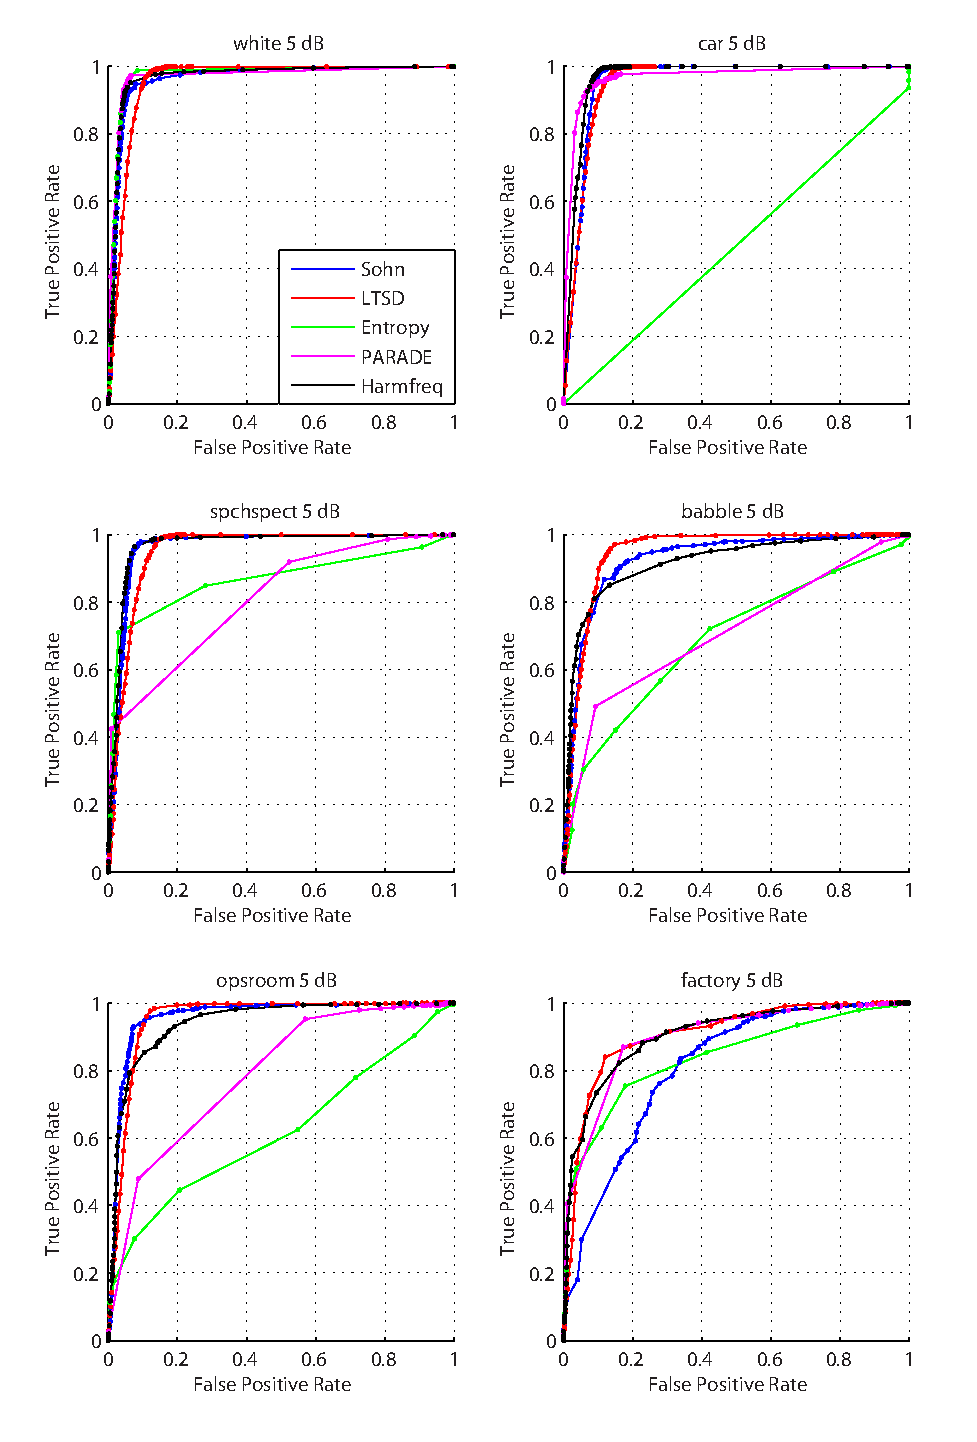
\includegraphics[width=1.0\columnwidth]{Figures/AppendixA/5dBh.pdf}
		\rule{37em}{0.5pt}
	\caption[ROC curves of the evaluated algorithms \emph{with} hang-over under 5 dB SNR]{ROC curves of the evaluated VAD algorithms \emph{with} hang-over under 5 dB SNR}
	\label{fig:5dBh}
\end{figure}

\begin{figure}[htbp]
	\centering
		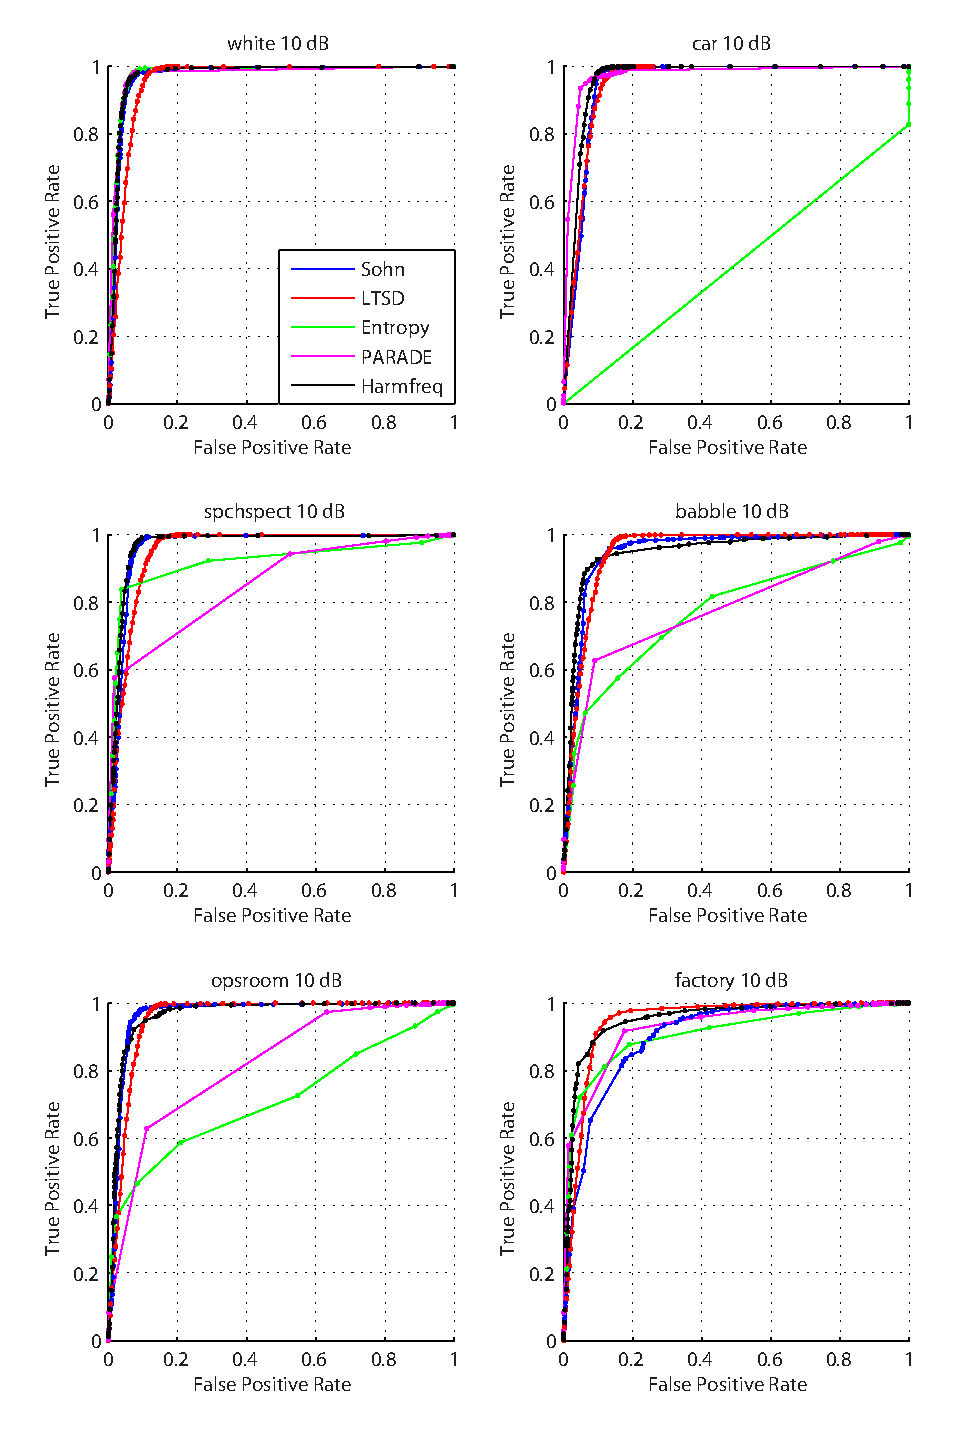
\includegraphics[width=1.0\columnwidth]{Figures/AppendixA/10dBh.pdf}
		\rule{37em}{0.5pt}
	\caption[ROC curves of the evaluated algorithms \emph{with} hang-over under 10 dB SNR]{ROC curves of the evaluated VAD algorithms \emph{with} hang-over under 10 dB SNR}
	\label{fig:10dBh}
\end{figure}

\begin{figure}[htbp]
	\centering
		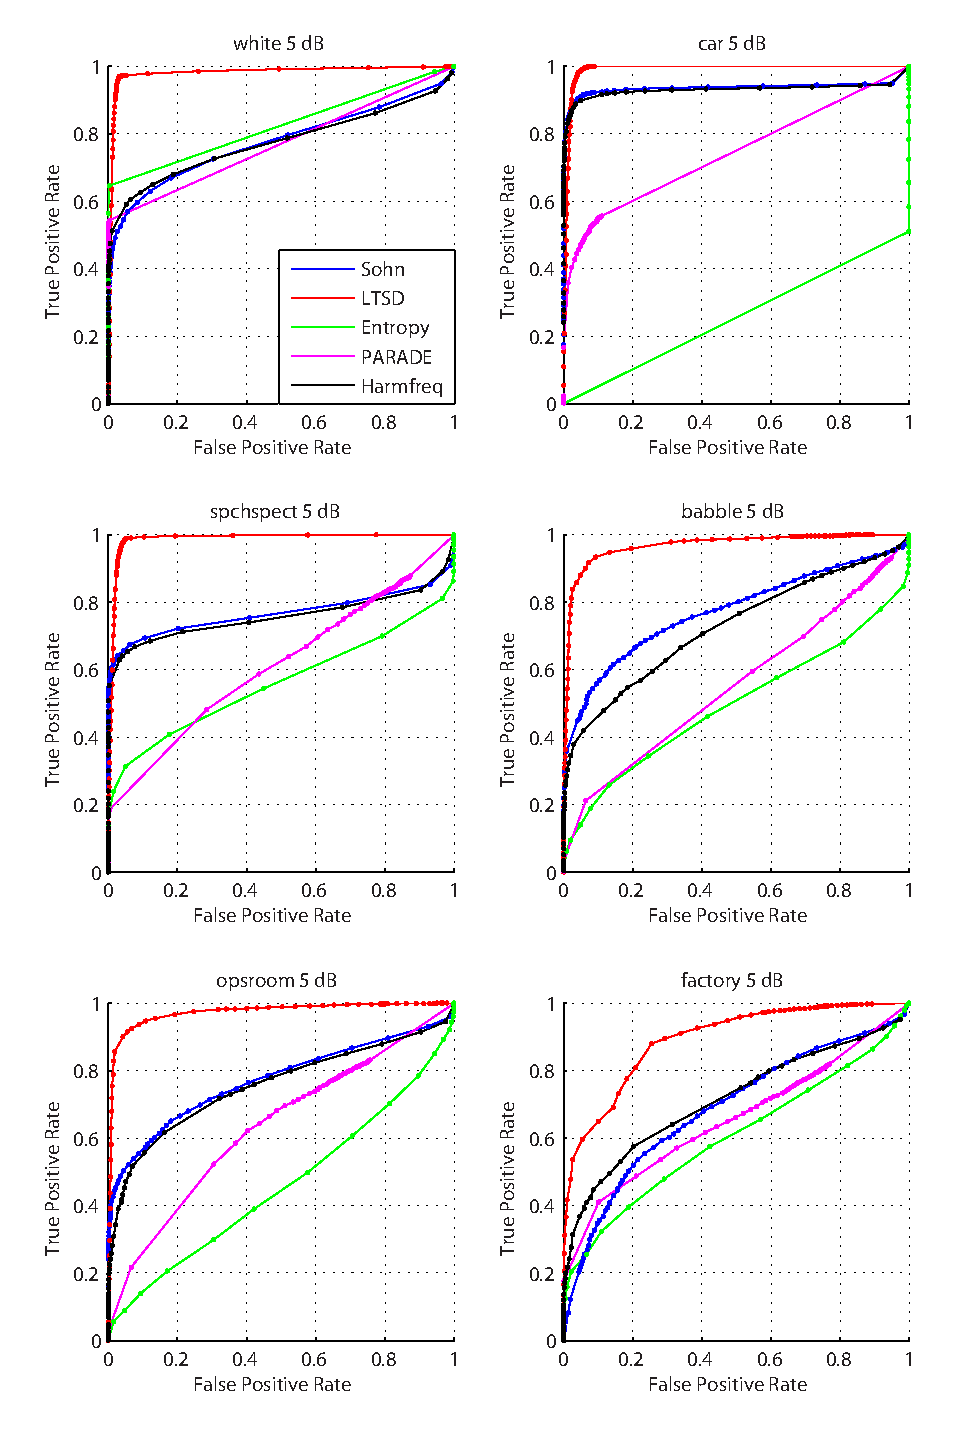
\includegraphics[width=1.0\columnwidth]{Figures/AppendixA/5dBnoh.pdf}
		\rule{37em}{0.5pt}
	\caption[ROC curves of the evaluated algorithms \emph{without} hang-over under 5 dB SNR]{ROC curves of the evaluated VAD algorithms \emph{without} hang-over under 5 dB SNR}
	\label{fig:5dBnoh}
\end{figure}

\begin{figure}[htbp]
	\centering
		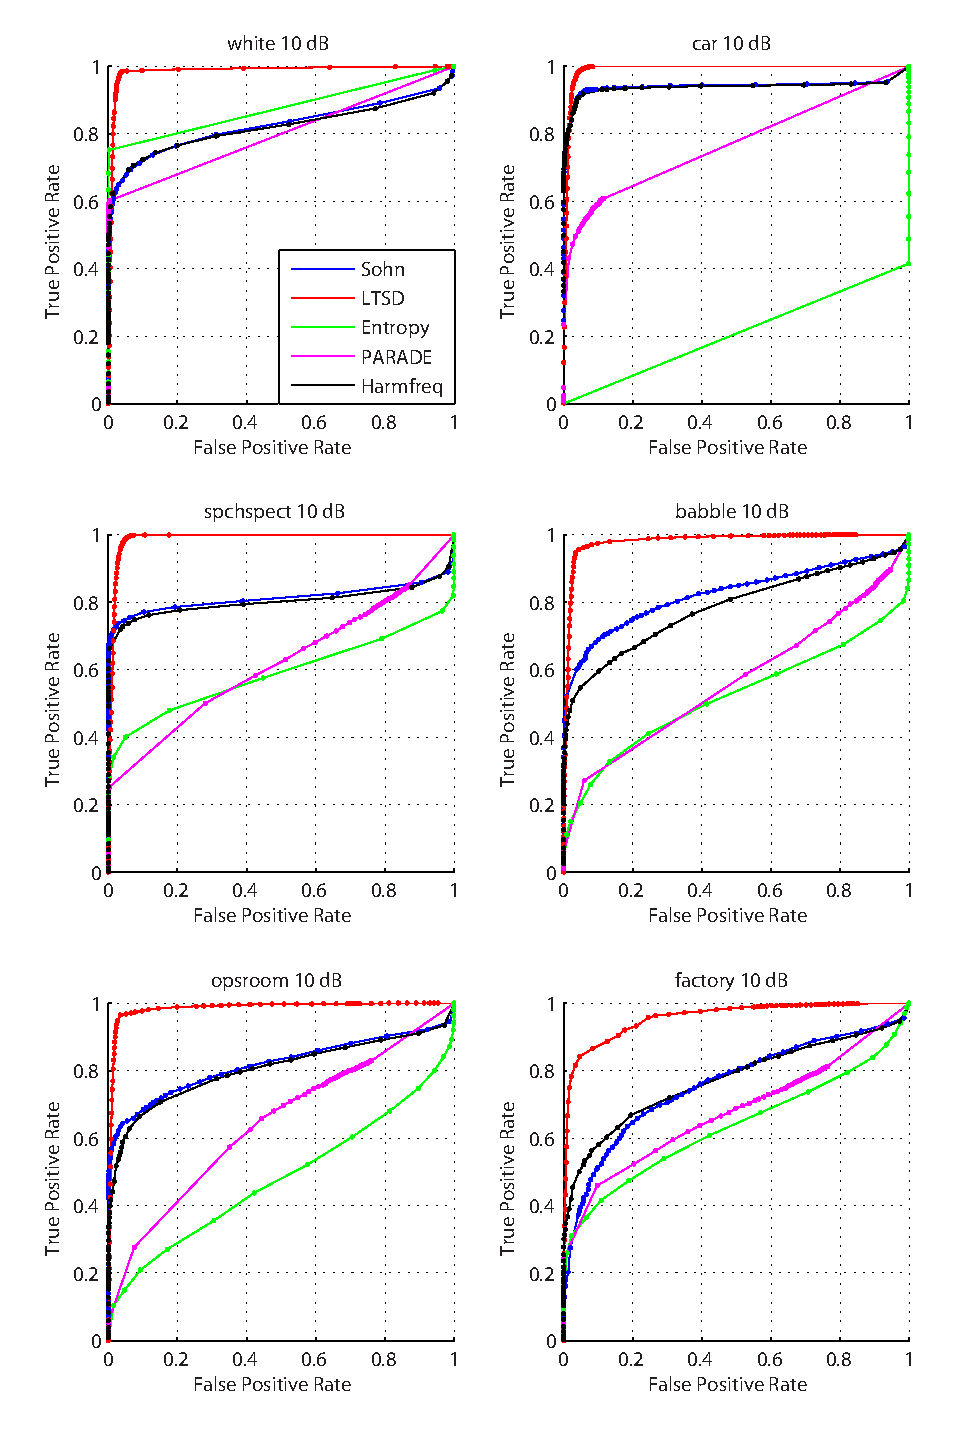
\includegraphics[width=1.0\columnwidth]{Figures/AppendixA/10dBnoh.pdf}
		\rule{37em}{0.5pt}
	\caption[ROC curves of the evaluated algorithms \emph{without} hang-over under 10 dB SNR]{ROC curves of the evaluated VAD algorithms \emph{without} hang-over under 10 dB SNR}
	\label{fig:10dBnoh}
\end{figure}

\begin{figure}[htbp]
	\centering
		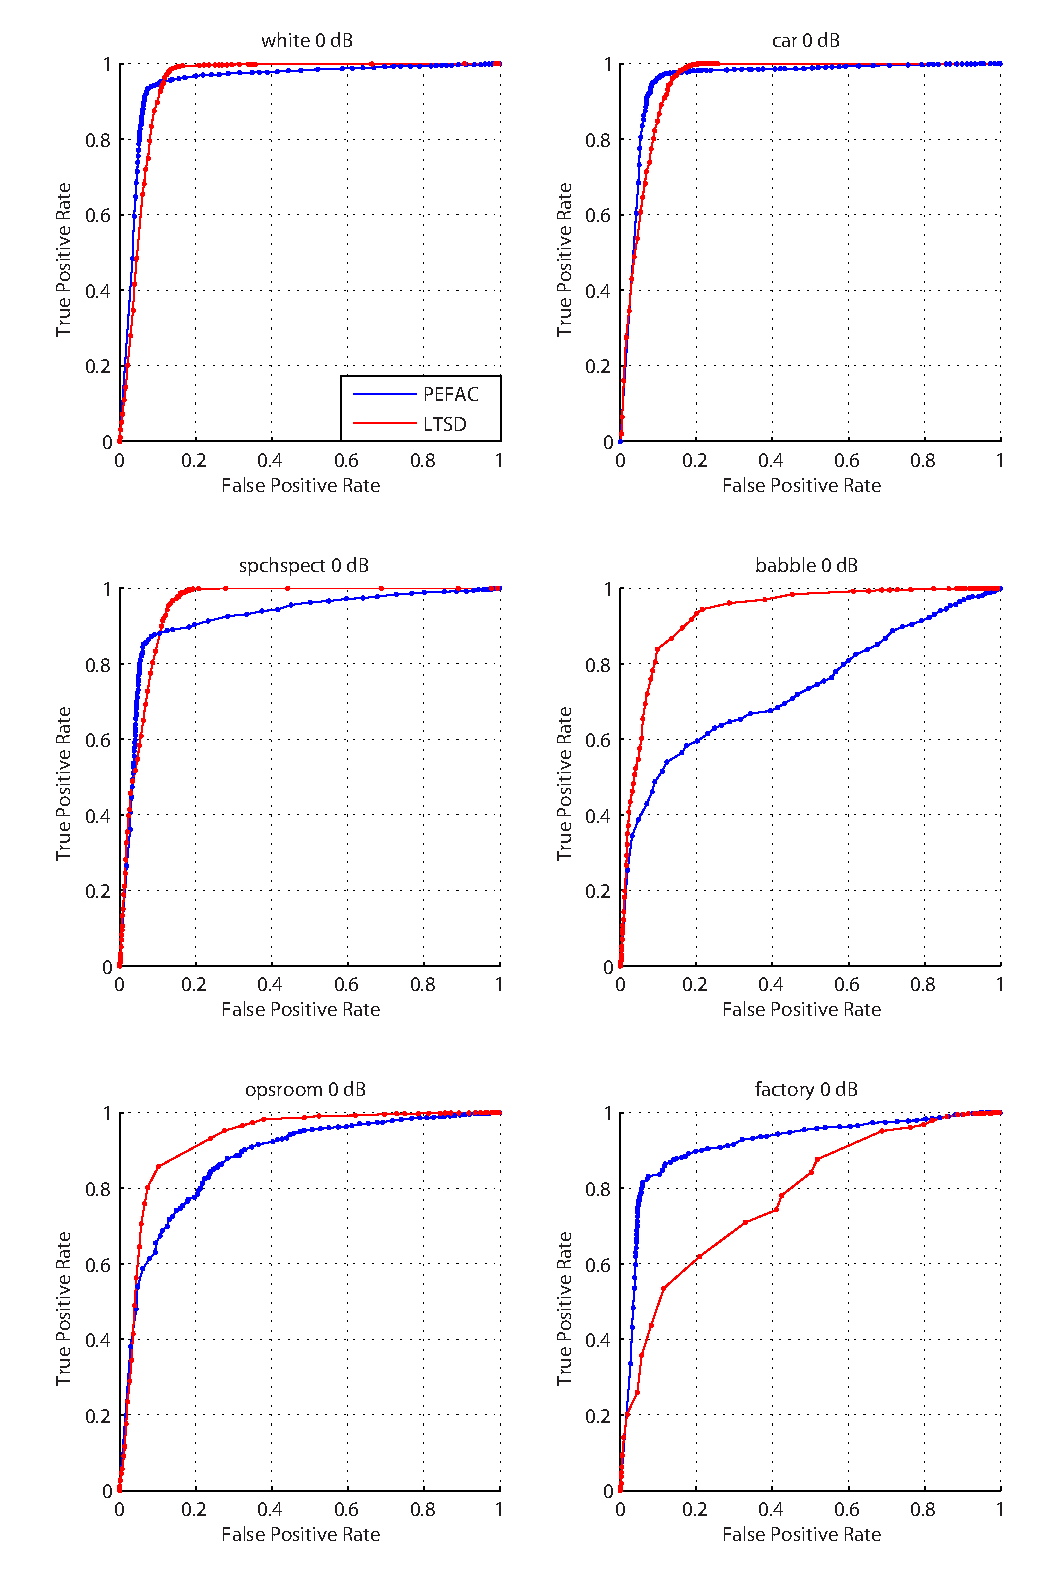
\includegraphics[width=1.0\columnwidth]{Figures/AppendixA/pefac0.pdf}
		\rule{37em}{0.5pt}
	\caption[ROC curves of PEFAC and LTSD \emph{with} hang-over under 0 dB SNR]{ROC curves of PEFAC and LTSD \emph{with} hang-over under 0 dB SNR}
	\label{fig:pefac0}
\end{figure}

\begin{figure}[htbp]
	\centering
		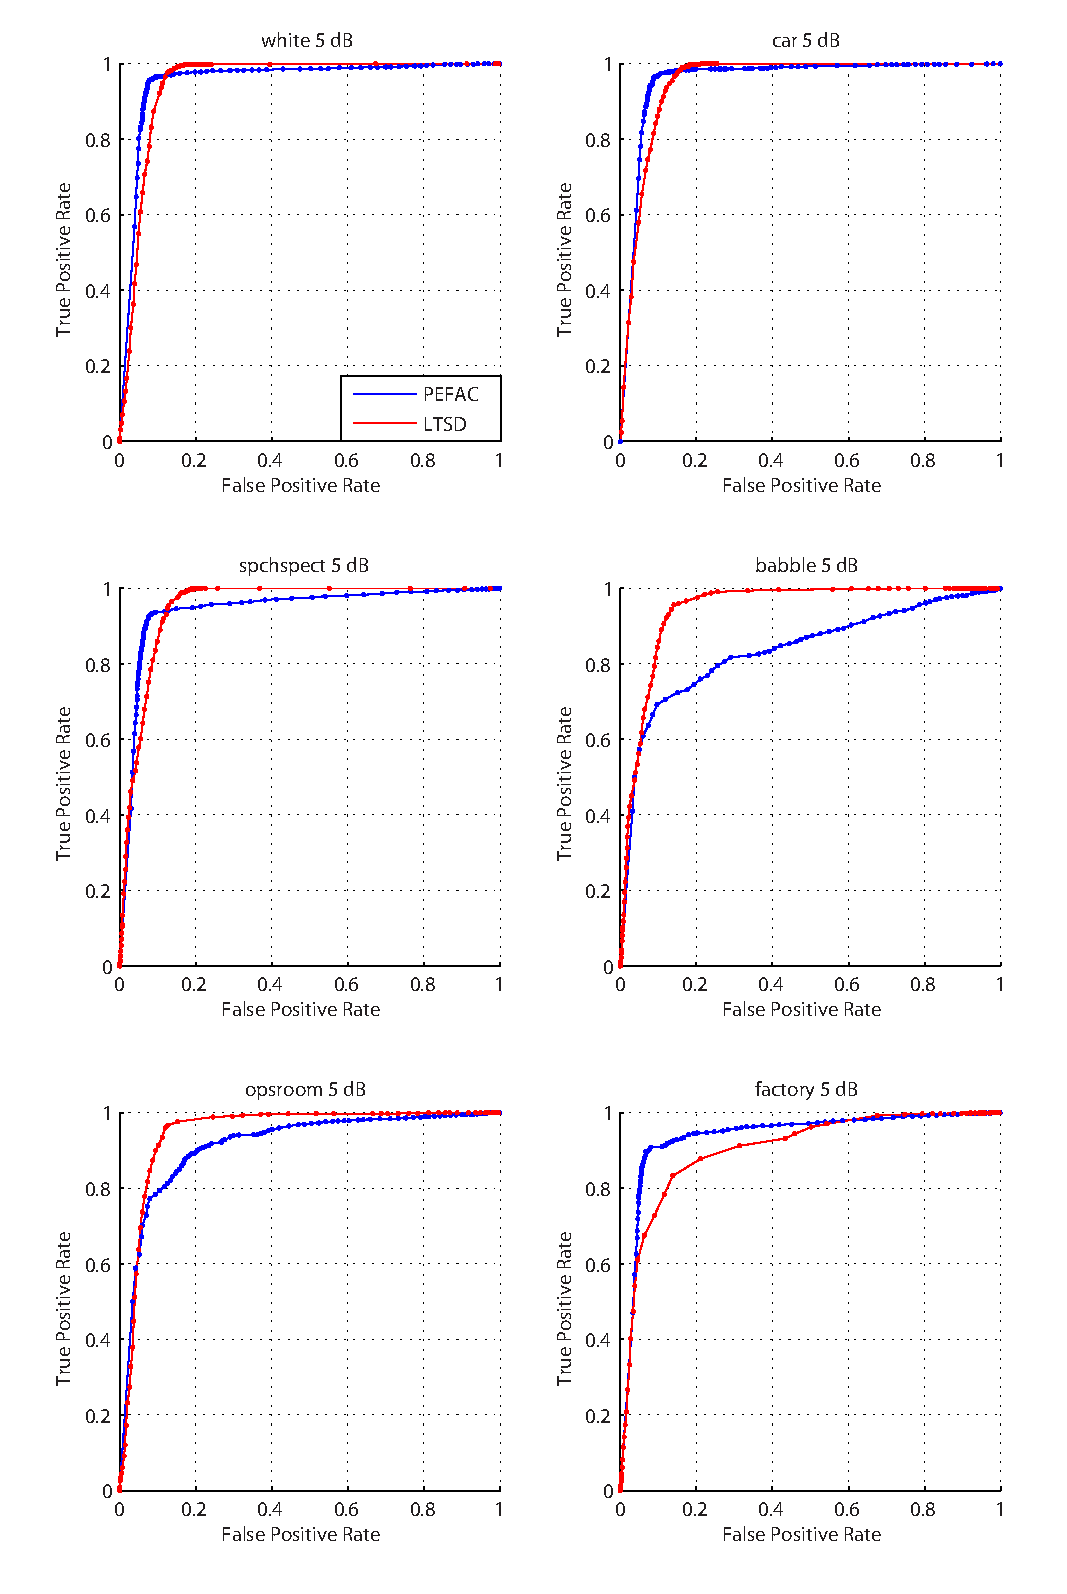
\includegraphics[width=1.0\columnwidth]{Figures/AppendixA/pefac5.pdf}
		\rule{37em}{0.5pt}
	\caption[ROC curves of PEFAC and LTSD \emph{with} hang-over under 5 dB SNR]{ROC curves of PEFAC and LTSD \emph{with} hang-over under 5 dB SNR}
	\label{fig:pefac5}
\end{figure}

\begin{figure}[htbp]
	\centering
		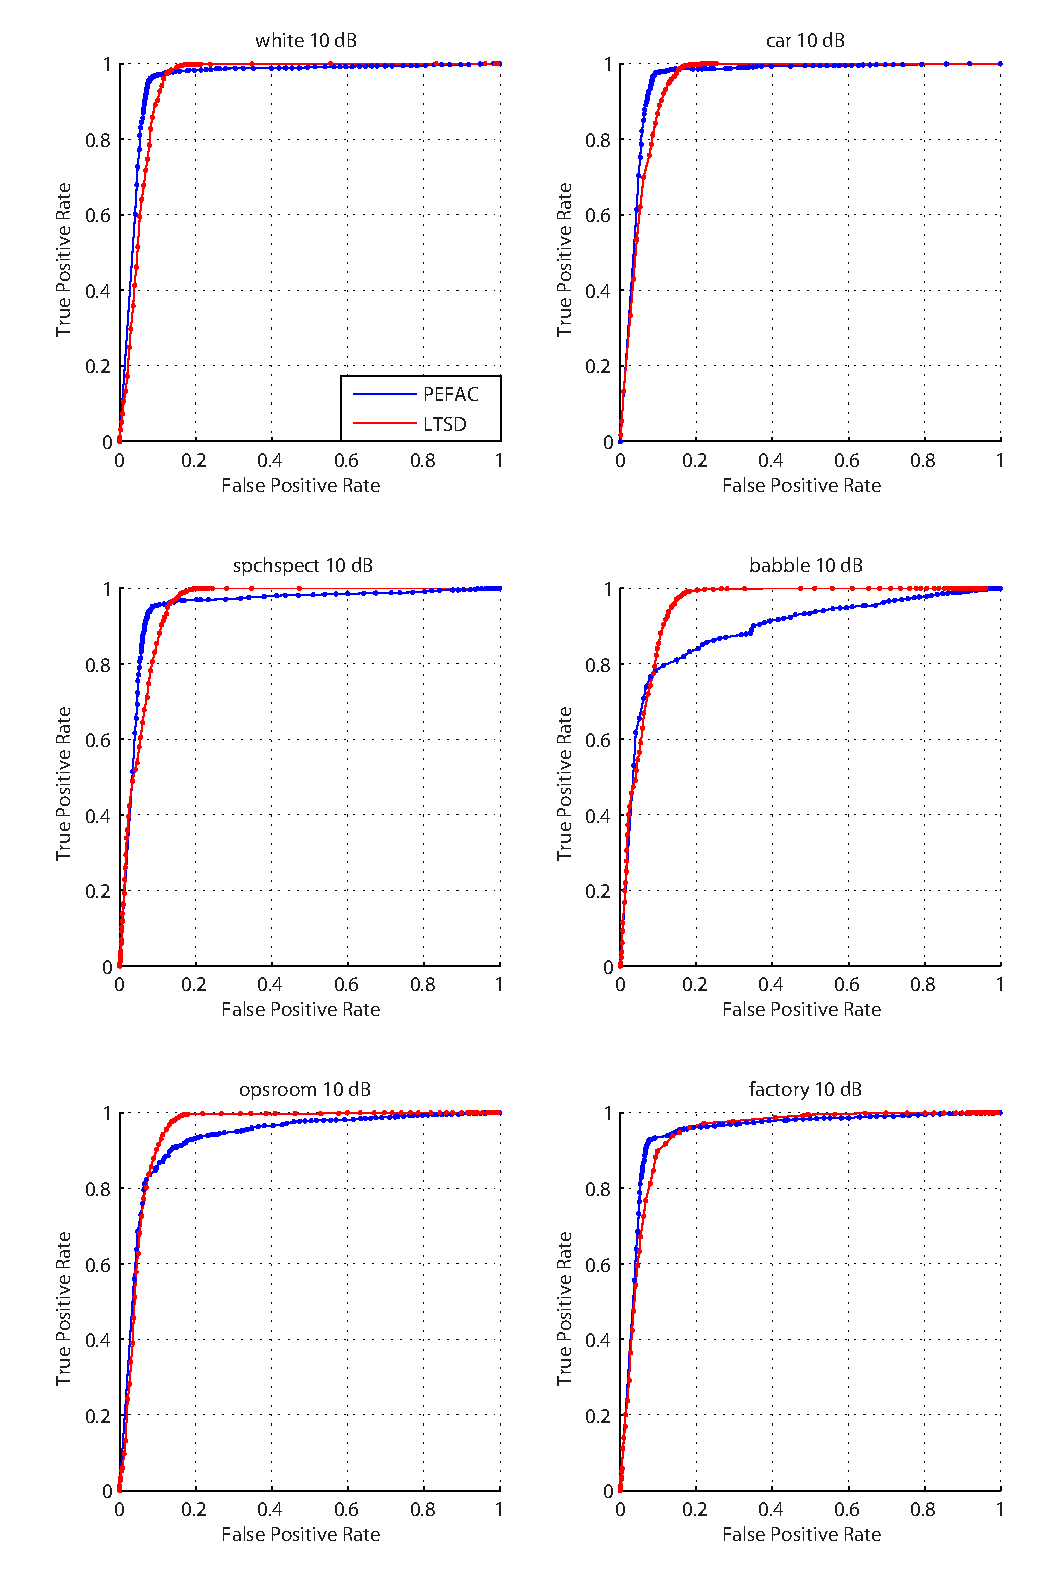
\includegraphics[width=1.0\columnwidth]{Figures/AppendixA/pefac10.pdf}
		\rule{37em}{0.5pt}
	\caption[ROC curves of PEFAC and LTSD \emph{with} hang-over under 10 dB SNR]{ROC curves of PEFAC and LTSD \emph{with} hang-over under 10 dB SNR}
	\label{fig:pefac10}
\end{figure}
%\input{Appendices/AppendixB}
%\input{Appendices/AppendixC}

\addtocontents{toc}{\vspace{1em}} % Add a gap in the Contents, for aesthetics

\backmatter

%----------------------------------------------------------------------------------------
%	BIBLIOGRAPHY
%----------------------------------------------------------------------------------------

\label{Bibliography}

\lhead{\emph{Bibliography}} % Change the page header to say "Bibliography"

\nocite{*} % Include also the uncited references

\bibliographystyle{unsrtnat} % Use the "unsrtnat" BibTeX style for formatting the Bibliography in alphabetical order

\bibliography{Bibliography} % The references (bibliography) information are stored in the file named "Bibliography.bib"

\end{document}  